\documentclass[journal]{IEEEtran}
% DRAFT v0.1 (2026-10-14). Every number in the text is a macro from numbers.tex, generated by
% src/paper/paper_numbers.py from the result files (each macro carries its source as a comment);
% table bodies are generated into tables/; figures by src/paper/make_figures.py.
\usepackage[utf8]{inputenc}
\usepackage[T1]{fontenc}
\usepackage{amsmath,amssymb}
\usepackage{graphicx}
\usepackage{booktabs}
\usepackage{multirow}
\usepackage{xcolor}
\usepackage{cite}
\usepackage{url}
\usepackage[hidelinks,hypertexnames=false]{hyperref}
\usepackage{algorithm}
\usepackage{algpseudocode}
\graphicspath{{figs/}}
% Generated by src/paper/paper_numbers.py -- do not edit by hand.
\newcommand{\inwsDelivered}{19,090}  % data/clean/inws_cycles.csv node 1 rows
\newcommand{\inwsMissing}{16,230}  % results/scoping/inws_outages.csv ALL.lost_slots
\newcommand{\inwsLoss}{46.0\%}  % inws_outages: lost/(lost+delivered)
\newcommand{\inwsOutages}{1,619}  % inws_outages ALL.events
\newcommand{\inwsOneSlotEvents}{47.3\%}  % inws_outages 1-slot event_share
\newcommand{\inwsOneSlotLost}{4.7\%}  % inws_outages 1-slot lost_share
\newcommand{\inwsDayEvents}{14}  % inws_outages >=1 day events
\newcommand{\inwsDayEventShare}{0.9\%}  % inws_outages >=1 day event_share
\newcommand{\inwsDayLost}{50.7\%}  % outage_ci.csv InWaterSense L=24 share_obs
\newcommand{\inwsDayLostLo}{29.4\%}  % outage_ci.csv bootstrap 2.5%
\newcommand{\inwsDayLostHi}{64.6\%}  % outage_ci.csv bootstrap 97.5%
\newcommand{\inwsSixLost}{68.5\%}  % outage_ci.csv InWaterSense L=6 share_obs
\newcommand{\inwsSixLostLo}{54.9\%}  % outage_ci.csv
\newcommand{\inwsSixLostHi}{77.2\%}  % outage_ci.csv
\newcommand{\inwsRhoNextOut}{$+0.27$}  % outage_ci.csv spearman
\newcommand{\inwsRhoNextUp}{$-0.20$}  % outage_ci.csv spearman
\newcommand{\weijaRhoNextOut}{$+0.02$}  % outage_ci.csv spearman
\newcommand{\weijaPNextOut}{0.88}  % outage_ci.csv spearman
\newcommand{\weijaPNextUp}{0.73}  % outage_ci.csv spearman
\newcommand{\inwsMaxOutageDays}{13.3}  % inws_outages.log max slots x 611 s
\newcommand{\weijaStreams}{9}  % weija_outages.csv rows
\newcommand{\weijaStreamsWord}{nine}  % weija_outages.csv rows (in words, for prose)
\newcommand{\weijaCondLoss}{15.4\%}  % weija_outages.csv conductivity loss
\newcommand{\weijaCondOutages}{42}  % weija_outages.csv conductivity events
\newcommand{\weijaCondDayLost}{82.9\%}  % weija_outages.csv conductivity
\newcommand{\weijaCondDayLostLo}{0.0\%}  % outage_ci.csv Weija
\newcommand{\weijaCondDayLostHi}{93.5\%}  % outage_ci.csv Weija
\newcommand{\weijaCondDayN}{3}  % outage_ci.csv Weija n outages >= 1 d
\newcommand{\weijaDayLostMin}{71.0\%}  % weija_outages.csv min over streams
\newcommand{\weijaDayLostMax}{100.0\%}  % weija_outages.csv max over streams
\newcommand{\weijaMaxOutageDays}{36.7}  % weija_outages.csv max
\newcommand{\loedFrames}{5,118,817}  % loed_full.log
\newcommand{\loedDevices}{8,503}  % loed_full.log
\newcommand{\loedGateways}{9}  % loed_full.log
\newcommand{\loedDevicesTwoHundred}{1,780}  % loed_full.log
\newcommand{\loedWellHeard}{179}  % loed_full.log
\newcommand{\loedRadioLoss}{9.6\%}  % loed_full.log
\newcommand{\loedCondLoss}{0.25}  % loed_full.log
\newcommand{\loedBursts}{56,276}  % loed_full.log
\newcommand{\loedBurstOne}{84\%}  % loed_full.log
\newcommand{\loedBurstFive}{99\%}  % loed_full.log (length 1 + 2-5)
\newcommand{\loedCoLoss}{19.2\%}  % loed_full.log
\newcommand{\loedCoLossBase}{18.2\%}  % loed_full.log
\newcommand{\loedCoLossLo}{16.7\%}  % loed_full.log
\newcommand{\loedCoLossHi}{19.5\%}  % loed_full.log
\newcommand{\loedFullGateways}{5}  % loed_full_gateways.csv availability >= 0.999
\newcommand{\uvaAvail}{98.72\%}  % uva_loss.log
\newcommand{\uvaSysOutages}{12}  % uva_loss.log
\newcommand{\uvaSysMedianH}{1.67}  % uva_loss.log
\newcommand{\uvaSysMaxH}{82.2}  % uva_loss.log
\newcommand{\uvaSysDayShare}{83\%}  % uva_loss.log
\newcommand{\uvaMissing}{58,211}  % uva_loss.log
\newcommand{\uvaSysShare}{28.4\%}  % uva_loss.log
\newcommand{\uvaRadioShare}{71.6\%}  % uva_loss.log
\newcommand{\uvaGwShare}{0.0\%}  % uva_loss.log
\newcommand{\uvaLoss}{4.5\%}  % uva_loss.log
\newcommand{\uvaRuns}{36,519}  % uva_loss.log
\newcommand{\uvaRunsOne}{89\%}  % uva_loss.log
\newcommand{\uvaGwCDays}{29.9}  % uva_loss.log gateway C outage hours / 24
\newcommand{\uvaRainDry}{9.18\%}  % uva_loss.log
\newcommand{\uvaRainWet}{9.21\%}  % uva_loss.log
\newcommand{\uvaRainPairs}{18}  % uva_loss.log
\newcommand{\uvaRainP}{0.64}  % uva_loss.log
\newcommand{\uvaSensors}{10}  % uva_loss_sensors.csv
\newcommand{\uvaSensorFourRadio}{3.08\%}  % uva_loss_sensors.csv sensor04 radio/(rx+missing)
\newcommand{\aicBestInws}{discrete lognormal}  % outage model AIC table
\newcommand{\aicGeomGapInws}{3,677}  % AIC(geometric) - AIC(best)
\newcommand{\aicBestWeija}{discrete power law}  % outage model AIC table
\newcommand{\aicGeomGapWeija}{120}  % AIC(geometric) - AIC(best)
\newcommand{\aicBestUva}{two-geometric mixture}  % outage model AIC table
\newcommand{\aicGeomGapUva}{43,915}  % AIC(geometric) - AIC(best)
\newcommand{\arqEightMin}{2.59$\times$}  % loss_handling.csv LoRaWAN arq/unconf energy, min over records x SF x p
\newcommand{\arqEightMax}{7.35$\times$}  % same, max
\newcommand{\arqThreeMin}{1.51$\times$}  % loss_handling.csv LoRaWAN arq3/unconf energy, min
\newcommand{\arqThreeMax}{2.94$\times$}  % same, max
\newcommand{\arqGainMin}{$+5.0$}  % arq - unconf delivered share at p_radio = 0.096, min (pp)
\newcommand{\arqGainMax}{$+7.9$}  % same, max (pp)
\newcommand{\backoffMin}{1.20$\times$}  % NB-IoT unconf / unconf_backoff energy, min over records x search time x p
\newcommand{\backoffMax}{6.53$\times$}  % same, max
\newcommand{\bufNbMin}{$-5.5$}  % NB-IoT arq_buffer vs unconf_backoff energy change, min (percent)
\newcommand{\bufNbMax}{$+15.3$}  % same, max
\newcommand{\bufLoMin}{$-14.6$}  % LoRaWAN arq_buffer vs unconf energy change, min (percent)
\newcommand{\bufLoMax}{$+25.6$}  % same, max
\newcommand{\batchSaveMin}{1.33$\times$}  % fair baseline / batch1h energy, min over all configurations
\newcommand{\batchSaveMax}{3.33$\times$}  % same, max
\newcommand{\batchWithinMin}{$-3.3$}  % batch1h - unconf within-1h share, min (pp)
\newcommand{\batchWithinMax}{$+7.3$}  % same, max (pp)
\newcommand{\nConfigs}{20}  % loss_handling.csv record x radio x p_radio
\newcommand{\inwSevenUnconfE}{61.6}  % InWaterSense SF7 unconf J/day
\newcommand{\inwSevenUnconfLife}{1.80}  % InWaterSense SF7 unconf lifetime (y)
\newcommand{\inwSevenArqE}{447.1}  % InWaterSense SF7 arq J/day
\newcommand{\inwSevenArqLife}{0.46}  % InWaterSense SF7 arq lifetime (y)
\newcommand{\inwSevenBatchE}{18.9}  % InWaterSense SF7 batch1h J/day
\newcommand{\inwSevenBatchLife}{2.65}  % InWaterSense SF7 batch1h lifetime (y)
\newcommand{\inwRecordLossSim}{46.1\%}  % replayed InWaterSense link: unconf lost share (record grid)
\newcommand{\chainCount}{9}  % results/revision/chains/chain_<9 chains>.csv (D5 rerun)
\newcommand{\chainCountWord}{nine}  % number of chains, in words for prose
\newcommand{\chainSites}{27}  % unique sites in the 9 chain files
\newcommand{\chainPairsMin}{53}  % ordered pairs per parameter, min
\newcommand{\chainPairsMax}{57}  % ordered pairs per parameter, max
\newcommand{\chainOutages}{300}  % median number of simulated gaps per pair x param x length
\newcommand{\chainRtWinT}{72\%}  % chains T 24 h: share of pairs where a neighbour method beats own data (real time)
\newcommand{\chainRtGainT}{$+6.5$}  % chains T 24 h: median relative real-time gain, pairs with positive baseline
\newcommand{\chainBfWinT}{93\%}  % chains T 24 h: share of pairs where the neighbour improves bridging
\newcommand{\chainBfGainT}{$+23.4$}  % chains T 24 h: median relative bridging gain, pairs with positive baseline
\newcommand{\chainDielBeatsPersistT}{84\%}  % chains T 24 h: share of pairs where own diel beats persistence
\newcommand{\chainRtWinDo}{30\%}  % chains DO 24 h: share of pairs where a neighbour method beats own data (real time)
\newcommand{\chainRtGainDo}{$-8.8$}  % chains DO 24 h: median relative real-time gain, pairs with positive baseline
\newcommand{\chainBfWinDo}{70\%}  % chains DO 24 h: share of pairs where the neighbour improves bridging
\newcommand{\chainBfGainDo}{$+10.3$}  % chains DO 24 h: median relative bridging gain, pairs with positive baseline
\newcommand{\chainDielBeatsPersistDo}{77\%}  % chains DO 24 h: share of pairs where own diel beats persistence
\newcommand{\chainExclSite}{14206694}  % the single site whose pairs are excluded
\newcommand{\chainRtWinPh}{9\%}  % chains pH 24 h: share of pairs where a neighbour method beats own data (real time)
\newcommand{\chainRtGainPh}{$-6.6$}  % chains pH 24 h: median relative real-time gain, pairs with positive baseline
\newcommand{\chainBfWinPh}{38\%}  % chains pH 24 h: share of pairs where the neighbour improves bridging
\newcommand{\chainBfGainPh}{$-0.2$}  % chains pH 24 h: median relative bridging gain, pairs with positive baseline
\newcommand{\chainDielBeatsPersistPh}{42\%}  % chains pH 24 h: share of pairs where own diel beats persistence
\newcommand{\chainRtWinEc}{23\%}  % chains EC 24 h: share of pairs where a neighbour method beats own data (real time)
\newcommand{\chainRtGainEc}{$-1.9$}  % chains EC 24 h: median relative real-time gain, pairs with positive baseline
\newcommand{\chainBfWinEc}{25\%}  % chains EC 24 h: share of pairs where the neighbour improves bridging
\newcommand{\chainBfGainEc}{$-2.2$}  % chains EC 24 h: median relative bridging gain, pairs with positive baseline
\newcommand{\chainDielBeatsPersistEc}{5\%}  % chains EC 24 h: share of pairs where own diel beats persistence
\newcommand{\chainGainExcluded}{3}  % 24 h pairs excluded from relative gains (zero baseline error)
\newcommand{\chainTolOneH}{97\%}  % chains: median over pairs x params of the best own-data real-time method within tolerance, 1 h
\newcommand{\chainTolDayMed}{31\%}  % chains: median over pairs x params of the best of ALL methods within tolerance, 24 h
\newcommand{\chainTolDayQ}{63\%}  % chains: 75th percentile of the same, 24 h
\newcommand{\eNbUnconf}{0.31}  % params.NBIOT N211 rai200 (J, module)
\newcommand{\eNbConf}{0.33}  % params.NBIOT N211 rai400 (J, module)
\newcommand{\eNbSearch}{2.22}  % P_RX_N211 x 10 s (J, module)
\newcommand{\pRxNb}{0.222}  % loss_handling.P_RX_N211 (W)
\newcommand{\eSfSevenUnconf}{0.244}  % model.lora_report_energy SF7 20 B unconfirmed (J, radio)
\newcommand{\eSfSevenConf}{0.164}  % model.lora_report_energy SF7 20 B confirmed success (J, radio)
\newcommand{\eSfTwelveUnconf}{0.729}  % model.lora_report_energy SF12 20 B unconfirmed (J, radio)
\newcommand{\eSfTwelveConf}{0.858}  % model.lora_report_energy SF12 20 B confirmed success (J, radio)
\newcommand{\rpfNb}{42}  % Radio(NB-IoT N211 RAI).readings_per_frame()
\newcommand{\rpfSfSeven}{18}  % Radio(LoRaWAN SF7).readings_per_frame()
\newcommand{\rpfSfTwelve}{3}  % Radio(LoRaWAN SF12).readings_per_frame()
\newcommand{\batteryKJ}{87.9}  % params.BATTERIES 6600 mAh x 3.7 V (kJ)
\newcommand{\hostOnMW}{69}  % params.P_HOST_ON (mW)
\newcommand{\weijaCondMaxDays}{7.5}  % weija_outages.csv conductivity max_outage_d
\newcommand{\weijaCondStepMin}{32.5}  % weija_outages.csv conductivity step_min
\newcommand{\inwsRhoP}{$p<0.001$}  % outage_ci.csv InWaterSense spearman, both p < 0.001 (asserted)
\newcommand{\weijaRhoNextUp}{$-0.06$}  % outage_ci.csv Weija spearman outage vs next up-run
\newcommand{\weijaCondSixLost}{88.9\%}  % outage_ci.csv Weija L=6 share_obs
\newcommand{\geomDayInws}{less than 0.001\%}  % outage_models.csv geom share24h_model InWaterSense (asserted < 1e-5)
\newcommand{\geomSixInws}{11.4\%}  % outage_models.csv geom share6h_model InWaterSense
\newcommand{\geomDayWeija}{36.9\%}  % outage_models.csv geom share24h_model Weija
\newcommand{\uvaSixLost}{27.1\%}  % uva_loss_runs.csv share of lost frames in runs >= 6 h
\newcommand{\uvaDayLost}{23.6\%}  % uva_loss_runs.csv share of lost frames in runs >= 24 h
\newcommand{\loedCondRatio}{2.6}  % loed_full.log P(loss|loss) / pooled radio loss
\newcommand{\aicWeijaLnGap}{1.7}  % outage_models.csv Weija AIC(lognormal) - AIC(power law)
\newcommand{\bufSevenMin}{$-14.6$}  % LoRaWAN SF7 arq_buffer vs unconf energy change, min over records x p (percent)
\newcommand{\bufSevenMax}{$+0.6$}  % same SF7, max (percent)
\newcommand{\bufTwelveMin}{$+7.8$}  % LoRaWAN SF12 arq_buffer vs unconf energy change, min over records x p (percent)
\newcommand{\bufTwelveMax}{$+25.6$}  % same SF12, max (percent)
\newcommand{\nbSearchTimes}{2.2, 10, 60}  % loss_handling.csv NB-IoT radio names (search time, s)
\newcommand{\inwSevenBufE}{52.7}  % InWaterSense SF7 arq_buffer J/day
\newcommand{\inwSevenBufLife}{1.93}  % InWaterSense SF7 arq_buffer lifetime (y)
\newcommand{\inwSevenArqThreeE}{175.5}  % InWaterSense SF7 arq3 J/day
\newcommand{\chainNaiveWinDo}{77\%}  % chains DO 24 h: share of pairs where a neighbour method beats persistence
\newcommand{\chainPersistDo}{9.07}  % chains DO 24 h: median over pairs of persistence error
\newcommand{\chainDielDo}{4.33}  % chains DO 24 h: median over pairs of own-diel error
\newcommand{\chainBestNbDo}{5.13}  % chains DO 24 h: median over pairs of best neighbour error
\newcommand{\chainNaiveWinPh}{36\%}  % chains pH 24 h: share of pairs where a neighbour method beats persistence
\newcommand{\chainPersistPh}{0.175}  % chains pH 24 h: median over pairs of persistence error
\newcommand{\chainDielPh}{0.125}  % chains pH 24 h: median over pairs of own-diel error
\newcommand{\chainBestNbPh}{0.149}  % chains pH 24 h: median over pairs of best neighbour error
\newcommand{\chainGaps}{1, 3, 6, 12, 24, 48, 72}  % chain files H_h values (h)
\newcommand{\weijaManyDecimals}{10.4\%}  % Weija conductivity, non-imputed: share of values with > 3 decimals
\newcommand{\weijaMaxDecimals}{14}  % Weija conductivity, non-imputed: most decimals in a value
\newcommand{\hostSleepMW}{0.12}  % params.P_HOST_SLEEP (mW)
\newcommand{\tSenseS}{5}  % params.T_SENSE typical (s awake per sample)
\newcommand{\nbPsmUW}{9.35}  % N211 PSM sleep power (uW)
\newcommand{\loraSleepUW}{148}  % LoRa radio sleep power (uW)
\newcommand{\vNode}{3.7}  % params.V_NODE (V)
\newcommand{\gofPmin}{0.005}  % bootstrap KS: smallest attainable p with B = 200
\newcommand{\gofGeomDInws}{0.48}  % gof_models InWaterSense geometric KS D
\newcommand{\gofBestDInws}{0.027}  % gof_models InWaterSense smallest KS D of the others
\newcommand{\gofGeomDUva}{0.26}  % gof_models UVA geometric KS D
\newcommand{\gofBestDUva}{0.008}  % gof_models UVA smallest KS D of the others
\newcommand{\gofWeijaLnP}{0.37}  % gof_models Weija EC lognormal p
\newcommand{\gofWeijaPlP}{0.64}  % gof_models Weija EC power-law p
\newcommand{\gofInwsN}{1,619}  % gof_models InWaterSense gaps
\newcommand{\gofUvaN}{36,519}  % gof_models UVA runs
\newcommand{\deepBridgeOneSaits}{65\%}  % deep: SAITS bridging 1 h, share within tolerance
\newcommand{\deepBridgeOneStem}{62\%}  % deep: StemGNN bridging 1 h, share within tolerance
\newcommand{\deepBridgeDaySaits}{25\%}  % deep: SAITS bridging 24 h, share within tolerance
\newcommand{\deepBridgeDayStem}{23\%}  % deep: StemGNN bridging 24 h, share within tolerance
\newcommand{\deepRtOneSaits}{57\%}  % deep: SAITS realtime 1 h, share within tolerance
\newcommand{\deepRtOneStem}{52\%}  % deep: StemGNN realtime 1 h, share within tolerance
\newcommand{\deepRtDaySaits}{18\%}  % deep: SAITS realtime 24 h, share within tolerance
\newcommand{\deepRtDayStem}{16\%}  % deep: StemGNN realtime 24 h, share within tolerance
\newcommand{\deepBridgeOneInterp}{97\%}  % deep: interpolation 1 h bridging, same gaps
\newcommand{\deepBridgeDayInterp}{31\%}  % deep: interpolation 24 h bridging, same gaps
\newcommand{\deepRtOneDiel}{91\%}  % deep: own diel 1 h real time, same gaps
\newcommand{\deepRtDayDiel}{29\%}  % deep: own diel 24 h real time, same gaps
\newcommand{\deepDayDoSaits}{4.3}  % deep: SAITS 24 h bridging DO median max error (%sat)
\newcommand{\deepDayDoInterp}{6.7}  % deep: interpolation, same
\newcommand{\deepDayPhSaits}{0.126}  % deep: SAITS 24 h bridging pH median max error
\newcommand{\deepDayPhInterp}{0.148}  % deep: interpolation, same
\newcommand{\deepDayBestAny}{55\%}  % deep file: best within-tolerance share of any estimator, any parameter, 24 h
\newcommand{\deepGaps}{48,455}  % deep: gap x parameter evaluations per model
\newcommand{\mcDraws}{100}  % energy_mc draws
\newcommand{\mcArqDearer}{100\%}  % energy_mc: LoRaWAN draws with ARQ dearer than unconfirmed
\newcommand{\mcArqLow}{1.8$\times$}  % energy_mc: LoRaWAN ARQ/unconf, lowest 2.5% quantile
\newcommand{\mcBatchCheapOther}{98\%}  % energy_mc: SF7/NB-IoT draws with batch cheaper than the fair baseline, min
\newcommand{\mcBatchCheapTwelveMin}{85\%}  % energy_mc: SF12 share, min over records
\newcommand{\mcBatchCheapTwelveMax}{93\%}  % energy_mc: SF12 share, max
\newcommand{\mcBatchTwelveHi}{1.24$\times$}  % energy_mc: SF12 batch/fair 97.5% quantile, max
\newcommand{\mcBufMedMin}{0.81$\times$}  % energy_mc: buffer/fair median, min over record x radio
\newcommand{\mcBufMedMax}{1.10$\times$}  % same, max
\newcommand{\mcBufLo}{0.50$\times$}  % energy_mc: buffer/fair 2.5% quantile, min
\newcommand{\mcBufHi}{2.08$\times$}  % energy_mc: buffer/fair 97.5% quantile, max
\newcommand{\mcNbArqMed}{1.01$\times$}  % energy_mc: NB-IoT ARQ/unconf median
\newcommand{\ugwLoraRatio}{3$\times$}  % Ugwuanyi 2021 Tab. 5 LoRaWAN 1.19 J vs model 0.448 J (44 B, SF7, host incl.)
\newcommand{\ugwNbRatio}{40$\times$}  % Ugwuanyi 2021 Tab. 5 NB-IoT 21.4 J vs model 0.539 J (44 B, RAI, host incl.)
\newcommand{\weijaEcMissing}{916}  % gap_cause_summary.json weija
\newcommand{\weijaNodeSilentShare}{84\%}  % gap_cause_summary.json weija
\newcommand{\weijaOtherStreamShare}{16\%}  % gap_cause_summary.json
\newcommand{\weijaLongAliveShare}{6\%}  % gap_cause_summary.json: slots of v0.1 gaps >= 6 h with another stream
\newcommand{\weijaNodeLoss}{13.9\%}  % gap_cause_weija_records.csv node record loss
\newcommand{\weijaNodeGaps}{31}  % gap_cause_weija_records.csv node record gaps
\newcommand{\weijaNodeDayLost}{81\%}  % gap_cause_weija_records.csv node record S(1 d)
\newcommand{\inwsWindowShare}{57\%}  % gap_cause_summary.json inws: lost slots inside node 2's window
\newcommand{\inwsNodeTwoSilent}{79\%}  % gap_cause_summary.json inws
\newcommand{\inwsSharedLong}{74\%}  % gap_cause_summary.json inws pi, gaps >= 6 h
\newcommand{\inwsSpecificLong}{26\%}  % 1 - pi, gaps >= 6 h
\newcommand{\inwsSpecificShort}{63\%}  % 1 - pi, gaps < 6 h
\newcommand{\offExpectedInws}{83\%}  % loss_B.csv InWaterSense SF7 f=0.5 buffer: delivered/expected
\newcommand{\offExpectedWeija}{92\%}  % loss_B.csv Weija (node record) SF7 f=0.5 buffer: delivered/expected
\newcommand{\offBufFairZero}{0.85}  % loss_B.csv InWaterSense SF7 buffer/unconf energy, f=0
\newcommand{\offBufFairHalf}{1.02}  % loss_B.csv InWaterSense SF7 buffer/unconf energy, f=0.5
\newcommand{\offRealisedWeija}{0.49}  % loss_B.csv: realised node-off share for nominal f = 0.1 (Weija has few long gaps)
\newcommand{\arqGainFullMin}{0.0}  % loss_A.csv InWaterSense LoRaWAN ARQ gain (pp), full, p_radio 0, SF7/SF12, all variants
\newcommand{\arqGainFullMax}{0.0}  % loss_A.csv same, max
\newcommand{\arqGainUniformMin}{0.1}  % loss_A.csv InWaterSense LoRaWAN ARQ gain (pp), uniform, p_radio 0, SF7/SF12, all variants
\newcommand{\arqGainUniformMax}{4.6}  % loss_A.csv same, max
\newcommand{\arqGainBurstMin}{6.5}  % loss_A.csv InWaterSense LoRaWAN ARQ gain (pp), burst, p_radio 0, SF7/SF12, all variants
\newcommand{\arqGainBurstMax}{7.7}  % loss_A.csv same, max
\newcommand{\arqLostPp}{46}  % loss_A.csv InWaterSense unconfirmed: lost share (pp)
\newcommand{\arqGainWeijaMax}{0.9}  % loss_A.csv Weija records: largest ARQ gain (pp) over models
\newcommand{\arqBufRatioMin}{0.67}  % loss_A.csv InWaterSense LoRaWAN buffer/unconf energy over models
\newcommand{\arqBufRatioMax}{1.08}  % same, max
\newcommand{\arqRatioMin}{2.3$\times$}  % loss_A.csv InWaterSense LoRaWAN ARQ/unconf energy over models, variants
\newcommand{\arqRatioMax}{7.3$\times$}  % same, max
\newcommand{\arqVOneZeroTwo}{7.3$\times$}  % loss_A.csv InWaterSense SF7 full: 8 tx, LoRaWAN 1.0.2 DR stepping
\newcommand{\arqVOneZeroFour}{6.8$\times$}  % loss_A.csv InWaterSense SF7 full: NbTrans 8, LoRaWAN 1.0.4
\newcommand{\ramLossTwo}{24\%}  % loss_C.csv InWaterSense RAM 2 KB: readings lost (max over radios/strategies)
\newcommand{\ramLossEight}{10\%}  % loss_C.csv InWaterSense RAM 8 KB: readings lost (max over radios/strategies)
\newcommand{\maxBufferKB}{22}  % loss_C.csv InWaterSense largest buffer (KB)
\newcommand{\flashJDayMax}{0.03}  % loss_C.csv: largest flash energy (J/day), worst case
\newcommand{\radioJDayMin}{9}  % loss_C.csv: smallest radio energy (J/day)
\newcommand{\drainTwelveMedH}{1.2}  % loss_C.csv InWaterSense SF12 buffer, duty-cycle drain: median clearance (h)
\newcommand{\drainTwelveMaxD}{63}  % same, longest clearance (days)
\newcommand{\drainTwelveLiveP}{25}  % same, p95 delay of live readings during backlogs (days)
\newcommand{\drainSevenMaxH}{64}  % loss_C.csv InWaterSense SF7 duty-cycle drain: longest clearance (h)
\newcommand{\kEverySlotSeven}{2.2$\times$}  % sweep_k_batch.csv InWaterSense SF7: probe every slot / K=6 h
\newcommand{\kEverySlotNb}{3.7$\times$}  % sweep_k_batch.csv InWaterSense NB-IoT: same
\newcommand{\kSixToDaySave}{12\%}  % sweep: SF7 energy saving K 6 -> 24 h
\newcommand{\kPninetySix}{20}  % sweep: SF7 p90 recovery latency at K = 6 h (h)
\newcommand{\kPninetyDay}{61}  % sweep: SF7 p90 recovery latency at K = 24 h (h)
\newcommand{\uvaMissThouVsFive}{2\%}  % lorawan_uva_counters.csv: missing frames, threshold 1,000 vs 5,000
\newcommand{\uvaDecreases}{1}  % lorawan_uva_counters.csv: frame-counter decreases
\newcommand{\uvaBinOutMax}{14}  % lorawan_uva_bins.csv: system outages at 5-min bins
\newcommand{\uvaBinOutMin}{8}  % lorawan_uva_bins.csv: system outages at 30-min bins
\newcommand{\uvaBinDayMin}{82\%}  % lorawan_uva_bins.csv: down-time share in >= 1 d outages, min over bins
\newcommand{\uvaBinDayMax}{84\%}  % same, max
\newcommand{\uvaBinSysMin}{28.0\%}  % lorawan_uva_bins.csv: system share of missing frames, min
\newcommand{\uvaBinSysMax}{28.6\%}  % same, max
\newcommand{\loedLossHundred}{10.0\%}  % lorawan_loed_counters.csv well-heard devices, reset threshold 100
\newcommand{\loedLossThousand}{10.9\%}  % same, threshold 1,000 (the analysis)
\newcommand{\loedResetDevices}{81}  % well-heard devices with a frame-counter reset
\newcommand{\loedWellHeardN}{179}  % well-heard devices
\newcommand{\usgsExcT}{0.20}  % tolerance_summary.csv T: USGS excellent (median over sites)
\newcommand{\tolTwoT}{0.20}  % tolerance_summary.csv T: L2 (median over sites)
\newcommand{\dayRangeT}{1.10}  % tolerance_summary.csv T: median daily range
\newcommand{\ampFiveT}{0.74}  % tolerance_summary.csv T: median 5 sigma
\newcommand{\ampEightT}{1.19}  % tolerance_summary.csv T: median 8 sigma
\newcommand{\realFiveT}{100\%}  % tolerance_summary.csv T: sites with a real 3-h change >= 5 sigma
\newcommand{\realEightT}{83\%}  % tolerance_summary.csv T: sites with a real 3-h change >= 8 sigma
\newcommand{\usgsExcDO}{4.7}  % tolerance_summary.csv DO: USGS excellent (median over sites)
\newcommand{\tolTwoDO}{2.0}  % tolerance_summary.csv DO: L2 (median over sites)
\newcommand{\dayRangeDO}{10.0}  % tolerance_summary.csv DO: median daily range
\newcommand{\ampFiveDO}{7.4}  % tolerance_summary.csv DO: median 5 sigma
\newcommand{\ampEightDO}{11.9}  % tolerance_summary.csv DO: median 8 sigma
\newcommand{\realFiveDO}{100\%}  % tolerance_summary.csv DO: sites with a real 3-h change >= 5 sigma
\newcommand{\realEightDO}{97\%}  % tolerance_summary.csv DO: sites with a real 3-h change >= 8 sigma
\newcommand{\usgsExcEC}{6.3}  % tolerance_summary.csv EC: USGS excellent (median over sites)
\newcommand{\tolTwoEC}{4.2}  % tolerance_summary.csv EC: L2 (median over sites)
\newcommand{\dayRangeEC}{12.0}  % tolerance_summary.csv EC: median daily range
\newcommand{\ampFiveEC}{7.4}  % tolerance_summary.csv EC: median 5 sigma
\newcommand{\ampEightEC}{11.9}  % tolerance_summary.csv EC: median 8 sigma
\newcommand{\realFiveEC}{93\%}  % tolerance_summary.csv EC: sites with a real 3-h change >= 5 sigma
\newcommand{\realEightEC}{93\%}  % tolerance_summary.csv EC: sites with a real 3-h change >= 8 sigma
\newcommand{\usgsExcPh}{0.20}  % tolerance_summary.csv pH: USGS excellent (median over sites)
\newcommand{\tolTwoPh}{0.10}  % tolerance_summary.csv pH: L2 (median over sites)
\newcommand{\dayRangePh}{0.25}  % tolerance_summary.csv pH: median daily range
\newcommand{\ampFivePh}{0.50}  % tolerance_summary.csv pH: median 5 sigma
\newcommand{\ampEightPh}{0.80}  % tolerance_summary.csv pH: median 8 sigma
\newcommand{\realFivePh}{60\%}  % tolerance_summary.csv pH: sites with a real 3-h change >= 5 sigma
\newcommand{\realEightPh}{37\%}  % tolerance_summary.csv pH: sites with a real 3-h change >= 8 sigma
\newcommand{\netZeroJitterN}{50}  % netsim.csv: smallest cell (SF7) in which, without jitter, under 5% of nodes recover within 72 h
\newcommand{\netSevenMedMin}{2}  % netsim SF7, 1-h jitter: median node clearance, min (h)
\newcommand{\netSevenMedMax}{9}  % same, max
\newcommand{\netSevenAllMax}{42}  % netsim SF7: last node clears (h), max over settings
\newcommand{\netSevenEnergyMax}{12.5$\times$}  % netsim SF7, 500 nodes: energy per node vs alone, max
\newcommand{\netTwelveNoAck}{29\%}  % netsim SF12: received but unacknowledged, max
\newcommand{\netTwelveRxOne}{1.0\%}  % netsim SF12: gateway RX1 duty use, max (limit 1%)
\newcommand{\netTwelveCleared}{93\%}  % netsim SF12, 1-d outage, 100 nodes: share recovered in 72 h
\newcommand{\recDayAll}{31\%}  % reconstruct_bootstrap.csv: best-of-all within tolerance, 24 h, pooled
\newcommand{\recDayAllLo}{18\%}  % chain-blocked 95% CI low
\newcommand{\recDayAllHi}{49\%}  % CI high
\newcommand{\recDayT}{9\%}  % reconstruct_bootstrap.csv T 24 h best-of-all
\newcommand{\recDayPh}{49\%}  % reconstruct_bootstrap.csv pH 24 h best-of-all
\newcommand{\recDayDO}{22\%}  % reconstruct_bootstrap.csv DO 24 h best-of-all
\newcommand{\recDayEC}{56\%}  % reconstruct_bootstrap.csv EC 24 h best-of-all
\newcommand{\lagPosDown}{64\%}  % pairs_spatial DO: downstream neighbours with lag > 0
\newcommand{\lagPosUp}{68\%}  % pairs_spatial DO: upstream neighbours with lag > 0
\newcommand{\pairKmMin}{2.8}  % pairs_spatial distance min (km)
\newcommand{\pairKmMax}{300}  % max (km)
\newcommand{\pairKmMed}{42}  % median (km)
\newcommand{\chOneDev}{12/12}  % an2023_verdicts.json CH1
\newcommand{\chTwoDev}{12/12}  % an2023_verdicts.json CH2
\newcommand{\chFourDev}{38/48}  % an2023_verdicts.json CH4
\newcommand{\chFiveDev}{48/48}  % an2023_verdicts.json CH5
\newcommand{\chSixDev}{12/12}  % an2023_verdicts.json CH6
\newcommand{\chSevenDev}{12/12}  % an2023_verdicts.json CH7
\newcommand{\chNineLOneDev}{48/48}  % an2023_verdicts.json CH9_L1
\newcommand{\chNineLThreeDev}{48/48}  % an2023_verdicts.json CH9_L3
\newcommand{\chTenLOneDev}{12/12}  % an2023_verdicts.json CH10_L1
\newcommand{\chTenLThreeDev}{12/12}  % an2023_verdicts.json CH10_L3
\newcommand{\plausibleDev}{99.8\%}  % an2023_verdicts.json: injected events within plausible ranges
\newcommand{\designSites}{30}  % design_site_eligibility.csv status ok
\newcommand{\designCandidates}{39}  % design_site_eligibility.csv rows
\newcommand{\hFourFailMinDev}{$-10.8$}  % an2023_picture L2 worst failing event - arq (pp)
\newcommand{\hFourFailMaxDev}{$-5.1$}  % an2023_picture L2 mildest failing event - arq (pp)
\newcommand{\hFiveDiffMinDev}{$-0.02$}  % an2023_picture L2 bounded - arq, min (pp)
\newcommand{\hFiveDiffMaxDev}{$+0.59$}  % an2023_picture L2 bounded - arq, max (pp)
\newcommand{\eventOverBatchMinDev}{1.00$\times$}  % an2023_energy event / batch, min
\newcommand{\eventOverBatchMaxDev}{1.02$\times$}  % an2023_energy event / batch, max
\newcommand{\arqOverEventMinDev}{1.41$\times$}  % an2023_energy arq / event, min
\newcommand{\arqOverEventMaxDev}{3.86$\times$}  % an2023_energy arq / event, max
\newcommand{\boundedOverBatchMinDev}{1.05$\times$}  % an2023_energy bounded / batch, min
\newcommand{\boundedOverBatchMaxDev}{1.34$\times$}  % an2023_energy bounded / batch, max
\newcommand{\arqOverBoundedMinDev}{1.32$\times$}  % an2023_energy arq / bounded, min
\newcommand{\arqOverBoundedMaxDev}{2.51$\times$}  % an2023_energy arq / bounded, max
\newcommand{\arqOverBoundedCiLowDev}{1.29$\times$}  % an2023_energy: lowest lower 95% CI bound of arq / bounded over link x radio
\newcommand{\levOneArqOverMinDev}{1.20$\times$}  % an2023_energy_levels L1 arq / bounded, min
\newcommand{\levOneArqOverMaxDev}{1.61$\times$}  % an2023_energy_levels L1 arq / bounded, max
\newcommand{\levTwoArqOverMinDev}{1.33$\times$}  % an2023_energy_levels L2 arq / bounded, min
\newcommand{\levTwoArqOverMaxDev}{2.54$\times$}  % an2023_energy_levels L2 arq / bounded, max
\newcommand{\levThreeArqOverMinDev}{1.40$\times$}  % an2023_energy_levels L3 arq / bounded, min
\newcommand{\levThreeArqOverMaxDev}{3.38$\times$}  % an2023_energy_levels L3 arq / bounded, max
\newcommand{\batchLagMinDev}{0.50}  % an2023_latency: batch - event (h), min over link x radio
\newcommand{\batchLagMaxDev}{0.50}  % an2023_latency: batch - event (h), max
\newcommand{\knownOneUnconfNoneDev}{33\%}  % an2023_known_within none SF7 unconf 1 h
\newcommand{\knownSixUnconfNoneDev}{57\%}  % an2023_known_within none SF7 unconf 6 h
\newcommand{\knownDayUnconfNoneDev}{57\%}  % an2023_known_within none SF7 unconf 24 h
\newcommand{\knownOneArqNoneDev}{33\%}  % an2023_known_within none SF7 arq_buffer 1 h
\newcommand{\knownSixArqNoneDev}{57\%}  % an2023_known_within none SF7 arq_buffer 6 h
\newcommand{\knownDayArqNoneDev}{57\%}  % an2023_known_within none SF7 arq_buffer 24 h
\newcommand{\knownOneBatchNoneDev}{21\%}  % an2023_known_within none SF7 batch1h 1 h
\newcommand{\knownSixBatchNoneDev}{57\%}  % an2023_known_within none SF7 batch1h 6 h
\newcommand{\knownDayBatchNoneDev}{57\%}  % an2023_known_within none SF7 batch1h 24 h
\newcommand{\knownOneEventNoneDev}{33\%}  % an2023_known_within none SF7 design 1 h
\newcommand{\knownSixEventNoneDev}{57\%}  % an2023_known_within none SF7 design 6 h
\newcommand{\knownDayEventNoneDev}{57\%}  % an2023_known_within none SF7 design 24 h
\newcommand{\knownOneBoundedNoneDev}{33\%}  % an2023_known_within none SF7 design_bounded_nf 1 h
\newcommand{\knownSixBoundedNoneDev}{57\%}  % an2023_known_within none SF7 design_bounded_nf 6 h
\newcommand{\knownDayBoundedNoneDev}{57\%}  % an2023_known_within none SF7 design_bounded_nf 24 h
\newcommand{\knownOneUnconfInwsDev}{12\%}  % an2023_known_within InWaterSense SF7 unconf 1 h
\newcommand{\knownSixUnconfInwsDev}{21\%}  % an2023_known_within InWaterSense SF7 unconf 6 h
\newcommand{\knownDayUnconfInwsDev}{21\%}  % an2023_known_within InWaterSense SF7 unconf 24 h
\newcommand{\knownOneArqInwsDev}{17\%}  % an2023_known_within InWaterSense SF7 arq_buffer 1 h
\newcommand{\knownSixArqInwsDev}{35\%}  % an2023_known_within InWaterSense SF7 arq_buffer 6 h
\newcommand{\knownDayArqInwsDev}{43\%}  % an2023_known_within InWaterSense SF7 arq_buffer 24 h
\newcommand{\knownOneBatchInwsDev}{11\%}  % an2023_known_within InWaterSense SF7 batch1h 1 h
\newcommand{\knownSixBatchInwsDev}{35\%}  % an2023_known_within InWaterSense SF7 batch1h 6 h
\newcommand{\knownDayBatchInwsDev}{44\%}  % an2023_known_within InWaterSense SF7 batch1h 24 h
\newcommand{\knownOneEventInwsDev}{18\%}  % an2023_known_within InWaterSense SF7 design 1 h
\newcommand{\knownSixEventInwsDev}{38\%}  % an2023_known_within InWaterSense SF7 design 6 h
\newcommand{\knownDayEventInwsDev}{44\%}  % an2023_known_within InWaterSense SF7 design 24 h
\newcommand{\knownOneBoundedInwsDev}{19\%}  % an2023_known_within InWaterSense SF7 design_bounded_nf 1 h
\newcommand{\knownSixBoundedInwsDev}{38\%}  % an2023_known_within InWaterSense SF7 design_bounded_nf 6 h
\newcommand{\knownDayBoundedInwsDev}{44\%}  % an2023_known_within InWaterSense SF7 design_bounded_nf 24 h
\newcommand{\chOneConf}{12/12}  % an2024_verdicts.json CH1
\newcommand{\chTwoConf}{12/12}  % an2024_verdicts.json CH2
\newcommand{\chFourConf}{39/48}  % an2024_verdicts.json CH4
\newcommand{\chFiveConf}{48/48}  % an2024_verdicts.json CH5
\newcommand{\chSixConf}{12/12}  % an2024_verdicts.json CH6
\newcommand{\chSevenConf}{12/12}  % an2024_verdicts.json CH7
\newcommand{\chNineLOneConf}{48/48}  % an2024_verdicts.json CH9_L1
\newcommand{\chNineLThreeConf}{48/48}  % an2024_verdicts.json CH9_L3
\newcommand{\chTenLOneConf}{12/12}  % an2024_verdicts.json CH10_L1
\newcommand{\chTenLThreeConf}{12/12}  % an2024_verdicts.json CH10_L3
\newcommand{\plausibleConf}{99.7\%}  % an2024_verdicts.json: injected events within plausible ranges
\newcommand{\confSites}{33}  % eligibility_2024.csv status ok
\newcommand{\hFourFailMinConf}{$-9.0$}  % an2024_picture L2 worst failing event - arq (pp)
\newcommand{\hFourFailMaxConf}{$-6.9$}  % an2024_picture L2 mildest failing event - arq (pp)
\newcommand{\hFiveDiffMinConf}{$-0.01$}  % an2024_picture L2 bounded - arq, min (pp)
\newcommand{\hFiveDiffMaxConf}{$+0.56$}  % an2024_picture L2 bounded - arq, max (pp)
\newcommand{\eventOverBatchMinConf}{1.00$\times$}  % an2024_energy event / batch, min
\newcommand{\eventOverBatchMaxConf}{1.02$\times$}  % an2024_energy event / batch, max
\newcommand{\arqOverEventMinConf}{1.41$\times$}  % an2024_energy arq / event, min
\newcommand{\arqOverEventMaxConf}{3.86$\times$}  % an2024_energy arq / event, max
\newcommand{\boundedOverBatchMinConf}{1.05$\times$}  % an2024_energy bounded / batch, min
\newcommand{\boundedOverBatchMaxConf}{1.28$\times$}  % an2024_energy bounded / batch, max
\newcommand{\arqOverBoundedMinConf}{1.34$\times$}  % an2024_energy arq / bounded, min
\newcommand{\arqOverBoundedMaxConf}{2.55$\times$}  % an2024_energy arq / bounded, max
\newcommand{\arqOverBoundedCiLowConf}{1.28$\times$}  % an2024_energy: lowest lower 95% CI bound of arq / bounded over link x radio
\newcommand{\levOneArqOverMinConf}{1.20$\times$}  % an2024_energy_levels L1 arq / bounded, min
\newcommand{\levOneArqOverMaxConf}{1.57$\times$}  % an2024_energy_levels L1 arq / bounded, max
\newcommand{\levTwoArqOverMinConf}{1.35$\times$}  % an2024_energy_levels L2 arq / bounded, min
\newcommand{\levTwoArqOverMaxConf}{2.58$\times$}  % an2024_energy_levels L2 arq / bounded, max
\newcommand{\levThreeArqOverMinConf}{1.40$\times$}  % an2024_energy_levels L3 arq / bounded, min
\newcommand{\levThreeArqOverMaxConf}{3.47$\times$}  % an2024_energy_levels L3 arq / bounded, max
\newcommand{\batchLagMinConf}{0.43}  % an2024_latency: batch - event (h), min over link x radio
\newcommand{\batchLagMaxConf}{0.50}  % an2024_latency: batch - event (h), max
\newcommand{\knownOneUnconfNoneConf}{34\%}  % an2024_known_within none SF7 unconf 1 h
\newcommand{\knownSixUnconfNoneConf}{58\%}  % an2024_known_within none SF7 unconf 6 h
\newcommand{\knownDayUnconfNoneConf}{58\%}  % an2024_known_within none SF7 unconf 24 h
\newcommand{\knownOneArqNoneConf}{34\%}  % an2024_known_within none SF7 arq_buffer 1 h
\newcommand{\knownSixArqNoneConf}{58\%}  % an2024_known_within none SF7 arq_buffer 6 h
\newcommand{\knownDayArqNoneConf}{58\%}  % an2024_known_within none SF7 arq_buffer 24 h
\newcommand{\knownOneBatchNoneConf}{21\%}  % an2024_known_within none SF7 batch1h 1 h
\newcommand{\knownSixBatchNoneConf}{58\%}  % an2024_known_within none SF7 batch1h 6 h
\newcommand{\knownDayBatchNoneConf}{58\%}  % an2024_known_within none SF7 batch1h 24 h
\newcommand{\knownOneEventNoneConf}{34\%}  % an2024_known_within none SF7 design 1 h
\newcommand{\knownSixEventNoneConf}{58\%}  % an2024_known_within none SF7 design 6 h
\newcommand{\knownDayEventNoneConf}{58\%}  % an2024_known_within none SF7 design 24 h
\newcommand{\knownOneBoundedNoneConf}{34\%}  % an2024_known_within none SF7 design_bounded_nf 1 h
\newcommand{\knownSixBoundedNoneConf}{58\%}  % an2024_known_within none SF7 design_bounded_nf 6 h
\newcommand{\knownDayBoundedNoneConf}{58\%}  % an2024_known_within none SF7 design_bounded_nf 24 h
\newcommand{\knownOneUnconfInwsConf}{12\%}  % an2024_known_within InWaterSense SF7 unconf 1 h
\newcommand{\knownSixUnconfInwsConf}{22\%}  % an2024_known_within InWaterSense SF7 unconf 6 h
\newcommand{\knownDayUnconfInwsConf}{22\%}  % an2024_known_within InWaterSense SF7 unconf 24 h
\newcommand{\knownOneArqInwsConf}{16\%}  % an2024_known_within InWaterSense SF7 arq_buffer 1 h
\newcommand{\knownSixArqInwsConf}{34\%}  % an2024_known_within InWaterSense SF7 arq_buffer 6 h
\newcommand{\knownDayArqInwsConf}{42\%}  % an2024_known_within InWaterSense SF7 arq_buffer 24 h
\newcommand{\knownOneBatchInwsConf}{11\%}  % an2024_known_within InWaterSense SF7 batch1h 1 h
\newcommand{\knownSixBatchInwsConf}{34\%}  % an2024_known_within InWaterSense SF7 batch1h 6 h
\newcommand{\knownDayBatchInwsConf}{43\%}  % an2024_known_within InWaterSense SF7 batch1h 24 h
\newcommand{\knownOneEventInwsConf}{18\%}  % an2024_known_within InWaterSense SF7 design 1 h
\newcommand{\knownSixEventInwsConf}{36\%}  % an2024_known_within InWaterSense SF7 design 6 h
\newcommand{\knownDayEventInwsConf}{44\%}  % an2024_known_within InWaterSense SF7 design 24 h
\newcommand{\knownOneBoundedInwsConf}{19\%}  % an2024_known_within InWaterSense SF7 design_bounded_nf 1 h
\newcommand{\knownSixBoundedInwsConf}{36\%}  % an2024_known_within InWaterSense SF7 design_bounded_nf 6 h
\newcommand{\knownDayBoundedInwsConf}{44\%}  % an2024_known_within InWaterSense SF7 design_bounded_nf 24 h
\newcommand{\designEventsConf}{7,548}  % 2024 injected events (all settings)
\newcommand{\detectStepFive}{67\%}  % 2024: median over sites of the share of step5 events detected
\newcommand{\detectStepEight}{91\%}  % 2024: median over sites of the share of step8 events detected
\newcommand{\detectRampFive}{13\%}  % 2024: median over sites of the share of ramp5 events detected
\newcommand{\detectRampEight}{65\%}  % 2024: median over sites of the share of ramp8 events detected
\newcommand{\detectAll}{58.2\%}  % 2024: share of injected events detected (pooled)
\newcommand{\faMedian}{0.8}  % 2024: median over sites of false alarms per parameter per 30 days
\newcommand{\faMean}{1.1}  % 2024: mean
\newcommand{\alarmsPerDay}{0.13}  % 2024: median node alarms per day (clean series)
\newcommand{\alarmsPerDayMean}{0.15}  % 2024: mean
\newcommand{\onsetUnconfKnownMax}{7.0\%}  % 2024 onset in outage: unconf known ever, max
\newcommand{\onsetBufKnownMin}{98.8\%}  % 2024: buffering known ever, min
\newcommand{\picInwsDoUnconf}{75.8\%}  % an2024 L2 InWaterSense SF7 DO unconf
\newcommand{\picInwsDoArq}{72.4\%}  % an2024 L2 InWaterSense SF7 DO arq_buffer
\newcommand{\nfRatioMin}{0.987}  % 2024 clean L2: newest-first / FIFO energy, min
\newcommand{\nfRatioMax}{1.007}  % 2024 clean L2: newest-first / FIFO energy, max
\newcommand{\sitesBothYears}{29}  % sites eligible in both years
\newcommand{\sitesOnlyConf}{4}  % sites eligible only in 2024
\newcommand{\hEightPreSite}{01467200}  % v0.1 pre_D4: the only site where newest-first fell short
\newcommand{\hEightPreMin}{99.998\%}  % v0.1 pre_D4: min within-tolerance share of newest-first, no outage
\newcommand{\fifoMinSfTwelve}{98.72\%}  % v0.1 summary_H8 FIFO min within-tolerance, SF12, no outage
\newcommand{\hFourPassVOne}{29/48}  % v0.1 summary_H4 (before the D5 fix)
\newcommand{\ackCostMin}{3\%}  % ack_variant: application / network energy - 1, min over link x radio
\newcommand{\ackCostMax}{18\%}  % same, max
\newcommand{\ackArqOverMin}{1.29$\times$}  % ack_variant: ARQ+buffer / bounded (application ACK), min
\newcommand{\ackArqOverMax}{2.00$\times$}  % same, max
\newcommand{\ackPicWorst}{$-0.02$}  % ack_variant: bounded (application ACK) - ARQ+buffer picture, worst median site (pp)

% generated table bodies: TeX's primitive input (expandable), so \bottomrule can follow inside a tabular
\makeatletter\newcommand{\tabin}[1]{\@@input #1 }\makeatother

\begin{document}

\title{Outage-Aware Reporting and Loss Recovery for Energy-Efficient River Water-Quality Telemetry over LPWANs}

\author{Kofi Sarpong Adu-Manu and Stephen Kwaku Azongo
\thanks{K.~S.~Adu-Manu and S.~K.~Azongo are with the Department of Computer Science, University of Ghana, Legon, Ghana. Corresponding author: K.~S.~Adu-Manu.}}

\markboth{Draft v0.2 (revision) --- not for distribution}{}
\maketitle

\begin{abstract}
Battery-powered river water-quality nodes lose data, yet retransmission, buffering and reconstruction are analysed for short, independent losses. This paper measures loss in four real systems, two water-quality deployments and two LoRaWAN networks. Losses separate into short radio losses and rarer long delivery gaps, which hold most of the missing data in the water-quality deployments; a geometric gap-length model fits worst on every record. Replayed through a measurement-parameterised LoRaWAN and NB-IoT energy model, retransmission recovers under a fifth of the missing readings even under optimistic retry timing, at \arqRatioMin--\arqRatioMax{} the energy of unconfirmed reporting on LoRaWAN, whereas buffering with back-off recovers every generated reading at an energy close to that of recovering nothing. Neither simple nor deep reconstruction keeps most day-long gaps within tolerance. Bounded event-driven batching combines hourly batches, immediate alarms, a bounded-error trigger and buffering with back-off. Tested with frozen rules on held-out data from \confSites{} river sites, it matches per-reading reporting on alarm latency and real-time picture, while per-reading retransmission uses \arqOverBoundedMinConf--\arqOverBoundedMaxConf{} as much energy. Recovery of many nodes after a shared outage needs randomised probes, and large SF12 cells are limited by the gateway's acknowledgements.
\end{abstract}

\begin{IEEEkeywords}
Delivery gaps, network outages, store-and-forward, ARQ, LoRaWAN, NB-IoT, energy efficiency, water-quality monitoring, data reconstruction, event detection.
\end{IEEEkeywords}

\section{Introduction}
\label{sec:intro}

\IEEEPARstart{R}{iver} and reservoir monitoring with in-situ sensor nodes has to work where field visits are expensive and power is scarce~\cite{adumanu2017survey,adumanu2020smart}. A typical node samples temperature (T), specific conductance (EC), dissolved oxygen (DO) and pH every 5--30~minutes and sends the readings over a cellular or low-power wide-area network (LPWAN). Such nodes lose data. The InWaterSense deployment on the Sitnica river in Kosovo delivered \inwsDelivered{} of its expected readings and missed \inwsMissing{} (\inwsLoss)~\cite{ahmedi2022dataset}; the CSIRO water-quality network in Australia averaged about 64\% delivery because the gateway's connection to the server ``was down occasionally''~\cite{ledinh2007design}; and deployment reports describe gateways that lose power every night~\cite{langendoen2006murphy}, sinks that stop reconnecting until someone reboots them~\cite{ingelrest2010sensorscope,brzozowski2018lessons}, outages lasting days to weeks~\cite{puluckul2025subarctic}, and prolonged outages of cellular backhaul in remote areas~\cite{zennaro2025kyrgyzstan}.

There are three standard responses to a lost reading. A node can \emph{retransmit} it until it is acknowledged (automatic repeat request, ARQ); it can \emph{buffer} it and \emph{backfill} it later; or the server can \emph{reconstruct} it from the node's own history or from neighbouring sites. Which response is right depends on how data are actually lost. Retransmission helps against a short radio fade but spends energy in vain against a gateway that is down for a day; reconstruction can fill a ten-minute gap but not a week. Yet the analyses behind these remedies assume losses that are short: estimation over lossy links is analysed with independent or short-memory (Markov fading) packet errors~\cite{sinopoli2004kalman,huang2019retransmit,huang2020harq}, and state-of-the-art imputation methods are evaluated on random masks or on simulated failures of a few hours~\cite{kong2014dataloss,cini2022grin,marisca2022spin,chang2023deepcs}. Kong et al.~\cite{kong2014dataloss} describe long losses caused by damaged or depleted nodes, but as named patterns, not as measured durations. How long real delivery gaps last, how much of the missing data they hold, and what that implies for the energy and timeliness of each remedy have not been measured for environmental telemetry.

The contribution of this paper is not a new retransmission or prediction primitive: ARQ, buffering, back-off, batching and error-bounded (dual-prediction) reporting are all established. It is an evidence-to-design chain for outage-aware, energy-efficient telemetry. Real delivery records are used to measure how long losses last and where the missing data are. The records are then replayed through a measurement-parameterised LPWAN energy model, with explicit bounds on what the records cannot tell (why a reading is missing, and when within a slot the network returned), to decide when retransmission, buffering, batching and reconstruction pay. Finally, the reporting design that follows from these findings is fixed on one year of river data and tested on a held-out year. Four research questions structure the paper:
\begin{enumerate}
\item[RQ1] In the records studied, how long are the gaps in delivery, how much of the missing data do long gaps hold, and is a geometric (memoryless) run-length model adequate?
\item[RQ2] Under these gaps, what do retransmission, buffering with back-off and batching each recover, and at what energy and delay on LoRaWAN and NB-IoT?
\item[RQ3] Can reconstruction, from a site's own history or from neighbouring sites on the same river, replace delivery during a gap?
\item[RQ4] Can one reporting scheme raise alarms as fast as per-reading reporting and keep the server's real-time picture within a stated tolerance as often, while using substantially less energy than per-reading retransmission, on data not used to design it?
\end{enumerate}

The contributions follow the chain.
\begin{itemize}
\item \emph{Empirical loss structure} (Sec.~\ref{sec:outages}). In four records, two water-quality deployments and two LoRaWAN networks, losses separate into short radio losses and rare long delivery gaps or system outages, and in the water-quality records gaps of 6~h or more hold most of the missing readings. A geometric run-length model is strongly unsupported relative to the alternatives tested, and fails worst in the long-gap tail that decides between remedies. Where the records allow it, the cause of the long gaps is examined: node-wide silence on the single-node record, and mostly a shared gateway or backhaul path on the two-node record.
\item \emph{Consequence analysis with explicit bounds} (Secs.~\ref{sec:handling} and \ref{sec:reconstruct}). Replaying the records shows that ARQ recovers under a fifth of the missing readings even under optimistic assumptions on retry timing, at \arqRatioMin--\arqRatioMax{} the energy of unconfirmed reporting on LoRaWAN, whereas buffering with probe back-off recovers every reading the node generated at an energy close to that of recovering nothing in the model, and within \mcBufLo--\mcBufHi{} of it under wide parameter uncertainty. The results are bracketed for the unknown cause of gaps, the timing of retries within a slot, finite storage and the duty cycle, the back-off cap, and many nodes recovering at once. For reconstruction, the evaluated estimators, from a site's own day--night (diel) pattern to two contemporary deep imputers, keep few day-long gaps within tolerance, and a test against the last value alone overstates the value of neighbouring sites.
\item \emph{An outage-aware reporting design, confirmed on held-out data} (Sec.~\ref{sec:design}). Bounded event-driven batching combines hourly batches, immediate uploads on a node-side alarm, a bounded-error trigger that mirrors the server's estimate, and buffering with back-off. It was developed on \designSites{} USGS river sites in 2023 and then evaluated, with its parameters and decision rules frozen, on \confSites{} sites in 2024.
\end{itemize}

\emph{Scope.} The loss evidence comes from four records, and the two water-quality records cannot fully separate a network outage from a node that stopped producing readings; the paper therefore speaks of delivery gaps, and treats buffering's recovery as an upper bound for gaps of unknown cause. Energy comes from a model parameterised by published measurements, not from hardware built for this study; the claims are ratios between strategies on the same radio, tested against wide parameter uncertainty. The design is evaluated per node, with a separate multi-node model of recovery after a shared outage.

The rest of the paper is organised as follows. Sec.~\ref{sec:related} reviews related work, and Sec.~\ref{sec:data} describes the data, models and assumptions. Secs.~\ref{sec:outages}--\ref{sec:design} answer RQ1--RQ4 in turn, and Sec.~\ref{sec:discussion} discusses practical guidance, validity and limitations.

\section{Related Work}
\label{sec:related}

How sensor networks lose data: Packet delivery in dense sensor networks varies widely between links and over time~\cite{zhao2003understanding}. Kong et al.~\cite{kong2014dataloss} analysed three real datasets with losses of 23--64\% and identified five loss patterns, from random loss to ``successive loss in a row'' when a node fails, without measuring durations. Deployment reports describe long gaps anecdotally: a gateway losing its server connection~\cite{ledinh2007design}, nightly gateway power loss~\cite{langendoen2006murphy}, sinks and modems that stop until reset~\cite{ingelrest2010sensorscope,brzozowski2018lessons}, and LoRaWAN outages of days to weeks~\cite{puluckul2025subarctic}. Public LoRaWAN datasets now allow loss to be measured from frame counters: LoED~\cite{bhatia2020loed} and a 16-month deployment at the University of Virginia (UVA)~\cite{nikseresht2025uva}.

Estimation and retransmission: Kalman filtering with intermittent observations was analysed under independent arrivals~\cite{sinopoli2004kalman}; remote estimation asks whether to retransmit a failed packet or send a fresh one under independent or Markov fading channels~\cite{huang2019retransmit,huang2020harq}, and the age of information formalises timeliness~\cite{yates2021aoi,sun2026overlapping}. Application-layer coding recovers LoRaWAN frames lost to the radio~\cite{marcelis2017dare}. None of these solutions addresses periods of days with no communication.

Reconstruction: Compressive and low-rank gathering~\cite{luo2009cdg,cheng2013stcdg,piao2014lowrank}, and deep spatio-temporal imputation with graph networks~\cite{cini2022grin,marisca2022spin,cao2020stemgnn,jing2024casper} or self-attention~\cite{du2023saits,nie2024imputeformer}, exploit spatial and temporal correlation. Their evaluations use random losses~\cite{chang2023deepcs} or simulated blocks of 1--4~h~\cite{cini2022grin,marisca2022spin}, without a per-site diel baseline, although many such signals have strong day--night cycles. River networks have a specific spatial structure along the flow~\cite{peterson2010mixed}.

Store-and-forward and energy: Node-side buffering is an established practice~\cite{ledinh2007design,langendoen2006murphy,mcdonald2007sendt,murphy2021arctic,puluckul2025subarctic}, as is gateway-side storage during backhaul outages~\cite{zennaro2025kyrgyzstan}; reports also note that draining a backlog can starve live traffic~\cite{ingelrest2010sensorscope} and that storage fails~\cite{murphy2021arctic}. LPWAN energy rests on measured LoRaWAN~\cite{casals2017lorawan} and NB-IoT~\cite{michelinakis2021dissecting,sorensen2022nbiot} profiles and models~\cite{azari2019nbiot,ugwuanyi2021developing}. Dual prediction transmits only when the server's prediction would leave a tolerance~\cite{dias2016survey,santini2006adaptive}, and it was recently combined with adaptive sampling under an energy budget~\cite{arnaiz2024adaptive}; it is used to suppress reports over reliable or independently lossy links.

What is missing is a quantitative comparison of these remedies in terms of energy, completeness, and timeliness under measured gap processes (Table~\ref{tab:related}). This study also reuses dual prediction for a different purpose: to make an hourly batch leave early when the server's estimate would leave tolerance.

\begin{table}[t]
\centering
\caption{Closest related work. Gap durations: measured from data, reported without measurement, assumed in a model, or simulated. All four: ARQ, buffering, batching, and reconstruction. --: not addressed.}
\label{tab:related}
\scriptsize
\setlength{\tabcolsep}{3pt}
\newcolumntype{L}[1]{>{\raggedright\arraybackslash}p{#1}}
\begin{tabular}{@{}L{2.25cm}L{1.55cm}L{1.85cm}L{1.0cm}L{0.95cm}@{}}
\toprule
Work & Gap durations & Remedies compared & Energy & Held-out test \\
\midrule
Kong~\cite{kong2014dataloss} & reported & reconstruction & -- & -- \\
Deployments~\cite{ledinh2007design,ingelrest2010sensorscope,murphy2021arctic,puluckul2025subarctic} & reported & buffering & -- & -- \\
Huang~\cite{huang2019retransmit,huang2020harq} & assumed & retransmission & -- & -- \\
GRIN, SPIN~\cite{cini2022grin,marisca2022spin} & simulated & reconstruction & -- & -- \\
Arnaiz~\cite{arnaiz2024adaptive} & -- & dual prediction & modelled & -- \\
This study & measured & all four & ratios & yes \\
\bottomrule
\end{tabular}
\end{table}

\section{Data and Models}
\label{sec:data}

\emph{Terms.} A \emph{reading} is one sampling cycle of a node: the four parameters taken at one instant, which travel together. Time is divided into \emph{slots} at the reporting cadence, one reading per slot. A \emph{delivery gap} is a run of consecutive slots for which no reading reached the server, whatever the cause. A \emph{system outage} is a delivery gap verified to affect every node of a network (its gateway, backhaul or server); a \emph{gateway outage} affects the nodes of one gateway; a \emph{radio loss} is a frame lost while the rest of the path worked. These terms are used with these meanings throughout.

\subsection{Delivery records}
\label{sec:data-records}
The study uses four real records of what a network delivered (Table~\ref{tab:records}).

\emph{InWaterSense} (Kosovo). Node~1 of the InWaterSense deployment on the Sitnica river~\cite{ahmedi2022dataset,ahmedi2021inwatersense} reported about every 611~s from May~2015 to January~2016. The node sends each parameter as a separate message, seconds apart; the messages of one sampling instant are grouped into a reading, and a slot counts as delivered if a reading arrived for it. The node delivered \inwsDelivered{} readings and missed \inwsMissing{} slots (\inwsLoss).

\emph{Weija} (Ghana). The Weija deployment~\cite{adumanu2020smart} logged \weijaStreams{} parameter streams from one node from October~2018 to March~2019. Only records not marked as imputed count as delivered. Gap statistics and models use the conductivity stream (\weijaCondStepMin-minute cadence), and the other streams are used to check that its pattern is typical and to examine the cause of its gaps (Sec.~\ref{sec:data-cause}). Even among the records not marked as imputed, \weijaManyDecimals{} of the conductivity values carry more than the three decimals the logger otherwise records (up to \weijaMaxDecimals), a sign of unflagged interpolation. Such values hide some short gaps, so counts of short gaps are lower bounds; long gaps are not affected.

\emph{UVA} (Virginia, USA). Ten LoRaWAN sensors reporting every 5~min through three gateways on The Things Network, from February~2024 to June~2025~\cite{nikseresht2025uva,nikseresht2025uvadata}. Missing frames are found from frame-counter gaps. A missing frame is classified as a \emph{system} loss if no sensor at all reached the database in its 10-minute bin (network server, internet or the operators' logging pipeline), as a \emph{gateway} loss if all of the sensor's serving gateways were silent, and as a \emph{radio} loss otherwise.

\emph{LoED} (London, UK). The LoRaWAN at the Edge Dataset~\cite{bhatia2020loed,bhatia2020loeddata} logs \loedFrames{} uplink frames from \loedDevices{} device addresses heard by \loedGateways{} gateways. The devices belong to other operators, so a frame counts as lost when no LoED gateway heard it, and most devices are simply far away. Only \emph{well-heard} devices are therefore used, those with at least 200 frames and a radio loss below 20\% (\loedWellHeard{} of \loedDevicesTwoHundred{}), as a proxy for a node's own link, and a missing frame is classified as a gateway loss if none of the device's serving gateways logged anything in that hour.

\emph{Frame counters.} Both LoRaWAN analyses count a frame once per device and frame counter, whichever gateways heard it and however often it was retransmitted. A counter decrease or a jump beyond a threshold (5{,}000 frames on UVA, 1{,}000 on LoED) is treated as a reset or rejoin, not as loss. On UVA, \uvaDecreases{} counter decrease occurred, no (sensor, counter) pair was received at two different times (no counter reuse), every sensor kept its 5-minute cadence in every month, and a threshold of 1{,}000 instead of 5{,}000 changes the count of missing frames by \uvaMissThouVsFive. On LoED, \loedResetDevices{} of the \loedWellHeardN{} well-heard devices show a reset, and their pooled loss is \loedLossHundred{} with a threshold of 100 and \loedLossThousand{} with 1{,}000.

\begin{table}[t]
\centering
\caption{Delivery records. Loss: share of expected readings (InWaterSense, Weija) or frames (UVA, LoED) that did not arrive. Gaps: runs of consecutive missing slots or frames. Lost in $\ge$1~d: share of the missing readings that fall in gaps of one day or more, $S(1~\mathrm{d})$ in (\ref{eq:share}). Weija: conductivity stream (\weijaDayLostMin--\weijaDayLostMax{} over all \weijaStreams{} streams). LoED: well-heard devices only (radio loss). GW: gateways.}
\label{tab:records}
\scriptsize
\setlength{\tabcolsep}{2.5pt}
\begin{tabular}{@{}lllrrr@{}}
\toprule
Record & Type & Slot & Loss & Gaps & Lost in $\ge$1~d \\
\midrule
InWaterSense & water quality & 611 s & \inwsLoss & \inwsOutages & \inwsDayLost \\
Weija & water quality & \weijaCondStepMin{} min & \weijaCondLoss & \weijaCondOutages & \weijaCondDayLost \\
UVA & LoRaWAN, 3 GW & 5 min & \uvaLoss & \uvaRuns & \uvaDayLost \\
LoED & LoRaWAN, 9 GW & varies & \loedRadioLoss & \loedBursts & -- \\
\bottomrule
\end{tabular}
\end{table}

\subsection{What the water-quality records say about the cause of a gap}
\label{sec:data-cause}
Neither water-quality record has a node status log, so a gap in which the network was down cannot be told apart directly from one in which the node produced nothing. Two partial checks are possible.

\emph{Weija: the node's other streams.} The node's sensors share one logger and one uplink. A conductivity slot in which another stream delivered a genuine reading (not imputed, at most three decimals, not on an interpolated line) had a live node and a working uplink. Of the \weijaEcMissing{} missing conductivity slots, \weijaNodeSilentShare{} were node-silent, with no genuine reading from any stream, and \weijaOtherStreamShare{} were conductivity-only gaps with the link up. In gaps of 6~h or more only \weijaLongAliveShare{} of the slots had another stream delivering: Weija's long gaps are silences of the whole node, which may be the node, its logger or its uplink. The node-level record (a slot is delivered if any stream delivered) loses \weijaNodeLoss{} of the slots in \weijaNodeGaps{} gaps, with \weijaNodeDayLost{} of the missing slots in gaps of a day or more, close to the conductivity record's \weijaCondDayLost{}.

\emph{InWaterSense: the second node.} Both InWaterSense nodes reached the server through one gateway with one GPRS link, housed in node~2's manhole~\cite{ahmedi2022dataset}. While node~2 was operating (May--August 2015, a window that holds \inwsWindowShare{} of node~1's missing slots), a node-1 gap during which node~2 kept delivering cannot be a gateway, GPRS or server outage. Node~2 was silent during \inwsNodeTwoSilent{} of node~1's missing slots, far more often than when node~1 delivered. Correcting for node~2's own, local rate of silence, gaps of 6~h or more were about \inwsSharedLong{} shared-cause (gateway, backhaul, server or a shared power failure) and \inwsSpecificLong{} specific to node~1, while gaps shorter than 6~h were \inwsSpecificShort{} node-specific, as radio losses would be.

These checks support reading most long gaps as failures of the path to the server, but they cannot rule out that some were nodes that stopped producing readings. Sec.~\ref{sec:handling} therefore treats buffering's recovery as an upper bound and repeats the replay with up to half of the long-gap slots reassigned to a node that was off.

\subsection{Gap-length models}
\label{sec:data-outages}
A delivery record is reduced to alternating \emph{up-runs} (consecutive delivered slots) and gaps (consecutive missing slots), in units of the record's slot. Let $k_1,\dots,k_n$ be the gap lengths and $h(k)$ the duration of a gap of $k$ slots. Because the quantity that matters for loss handling is where the missing data are, not where the gap events are, the main statistic is the share of missing slots that fall in gaps of at least a duration $L$,
\begin{equation}
S(L)=\frac{\sum_{i:\,h(k_i)\ge L} k_i}{\sum_{i=1}^{n} k_i},
\label{eq:share}
\end{equation}
reported for $L=6$~h and 1~day with bootstrap 95\% confidence intervals~\cite{efron1979bootstrap} (gaps resampled with replacement, 5{,}000 draws). A gap is bounded by delivered slots on both sides, so every gap length is fully observed; only the first and last up-runs are censored, and up-runs are not modelled.

Four models are fitted to the gap lengths $k\ge1$ by maximum likelihood:
\begin{align}
P_\mathrm{geo}(k)&=(1-q)\,q^{k-1}, \label{eq:geo}\\
P_\mathrm{mix}(k)&=w\,(1-q_1)\,q_1^{k-1}+(1-w)\,(1-q_2)\,q_2^{k-1}, \label{eq:mix}\\
P_\mathrm{ln}(k)&=\frac{\Phi\!\left(\frac{\ln(k+\frac12)-\mu}{\sigma}\right)-\Phi\!\left(\frac{\ln(k-\frac12)-\mu}{\sigma}\right)}{1-\Phi\!\left(\frac{\ln\frac12-\mu}{\sigma}\right)}, \label{eq:ln}\\
P_\mathrm{pl}(k)&=\frac{k^{-\alpha}}{\zeta(\alpha)}, \label{eq:pl}
\end{align}
where $\Phi$ is the standard normal distribution function and $\zeta$ the Riemann zeta function. The geometric model (\ref{eq:geo}) is the distribution of gap lengths whenever the loss process has a single loss state with a constant chance of ending in each slot: independent (Bernoulli) losses, and the two-state Gilbert--Elliott channel, whose losses are correlated in time but whose loss periods still have geometric lengths. It is this single-loss-state assumption on gap lengths that is tested here. The two-geometric mixture (\ref{eq:mix}) is equivalent to a Markov chain with one up state and two loss states (``short loss'' and ``long gap''); (\ref{eq:ln}) is a lognormal discretised to integer lengths; and (\ref{eq:pl}) is a discrete power law. Models are compared by Akaike's information criterion, $\mathrm{AIC}=2p-2\ln\hat{\mathcal{L}}$ for $p$ parameters and maximised likelihood $\hat{\mathcal{L}}$~\cite{akaike1974aic}, lower being better. Because AIC only ranks models, each is also tested absolutely, by a discrete Kolmogorov--Smirnov statistic $D=\max_k|\hat F(k)-F(k)|$ with a parametric-bootstrap $p$-value (200 samples from the fitted model, each refitted). Dependence between consecutive gaps and up-runs is measured by Spearman's rank correlation.

\subsection{Energy model and loss-handling strategies}
\label{sec:data-energy}
The node is a Libelium Waspmote-class host~\cite{libelium2020plugsense} with one of three radios: NB-IoT (the N211 module measured in~\cite{michelinakis2021dissecting}, with release assistance, RAI), LoRaWAN at spreading factor 7 (SF7), or LoRaWAN at SF12 in the EU868 band. Each transmission attempt $a$ is charged the measured energy $e_a$ of its radio and outcome:

\emph{NB-IoT.} The measurements~\cite{michelinakis2021dissecting} send UDP datagrams of 12--512~B in normal coverage to a server that echoes them, without an application protocol such as CoAP. An unconfirmed report costs \eNbUnconf~J (connection released after the uplink) and a confirmed one \eNbConf~J (released after the server's echo, which is the acknowledgement: it comes from the application, end to end). A bulk frame of up to 512~B, the module's largest datagram, costs up to 60\% more than a 20-byte report~\cite{michelinakis2021dissecting}. No published measurement was found of the energy that an NB-IoT modem spends searching for a cell when there is no network; it is therefore modelled as the receive power of \pRxNb~W~\cite{sorensen2022nbiot} times a search time $T_\mathrm{search}$, swept over $\{2.2, 10, 60\}$~s (default 10~s, \eNbSearch~J per failed attempt).

\emph{LoRaWAN.} Energies come from the state-by-state current profile of~\cite{casals2017lorawan}, with airtime computed from the payload. At SF7 the acknowledgement arrives in the first receive window, so a confirmed success (\eSfSevenConf~J for a 20-byte report) is cheaper than an unconfirmed report (\eSfSevenUnconf~J), which keeps both windows open; at SF12 it arrives in the second window and a confirmed success is dearer (\eSfTwelveConf{} vs \eSfTwelveUnconf~J). A failed confirmed attempt adds the retransmission time-out, RETRANSMIT\_TIMEOUT, of 1--3~s~\cite{lora2021rp002}. The number of transmissions depends on the specification version. LoRaWAN 1.0.2 strongly recommends eight transmissions of a confirmed frame, with the data rate lowered every two~\cite{lora2016spec102}; LoRaWAN 1.0.4 transmits a frame NbTrans times, a number between 1 and 15 set by the network, with no change of data rate~\cite{lora2020spec104}. Both are evaluated. The acknowledgement of a confirmed uplink comes from the network server; Sec.~\ref{sec:des-design} returns to what this means for the design. Frames carry at most the regional maximum payload~\cite{lora2021rp002}, and the 1\% duty cycle forbids a new frame before 100 times the previous frame's airtime has passed.

A reading in a bulk frame takes 12~B (four parameters, a time offset and a sequence number) and a frame 4~B of overhead, so a frame holds \rpfNb{} readings on NB-IoT, \rpfSfSeven{} at SF7 and \rpfSfTwelve{} at SF12. The host is awake for every attempt, at $P_\mathrm{on}=\hostOnMW$~mW~\cite{libelium2020plugsense}, and its awake time is added to $e_a$. Over a record of $D$ days with sampling interval $T_\mathrm{s}$ (s), the transmission energy per day and the modelled lifetime on a battery of energy $B$ are
\begin{gather}
E_\mathrm{tx}=\frac{1}{D}\sum_{a} e_a,\qquad Y=\frac{B}{365\,(E_\mathrm{floor}+E_\mathrm{tx})},\label{eq:energy}\\
E_\mathrm{floor}=86{,}400\,(P_\mathrm{sleep}^\mathrm{radio}+P_\mathrm{sleep}^\mathrm{host})+\frac{86{,}400}{T_\mathrm{s}}\,P_\mathrm{on}\,T_\mathrm{sense},\label{eq:floor}
\end{gather}
where the floor (\ref{eq:floor}) covers sleep and sensing: radio sleep power \nbPsmUW~$\mu$W for NB-IoT in power-saving mode~\cite{michelinakis2021dissecting} and \loraSleepUW~$\mu$W for the LoRa radio~\cite{casals2017lorawan}, host deep sleep \hostSleepMW~mW~\cite{libelium2020plugsense}, and an assumed $T_\mathrm{sense}=\tSenseS$~s awake per sample for probe settling and reading, with a 6{,}600~mAh battery at \vNode~V ($B=\batteryKJ$~kJ). Absolute energy depends strongly on the platform and the protocol stack: an independent measurement on a different board and stack~\cite{ugwuanyi2021developing} (a 44-byte uplink, TCP without RAI on NB-IoT) reports \ugwLoraRatio{} the per-message energy of this model for LoRaWAN SF7 and \ugwNbRatio{} for NB-IoT. The results are therefore stated as ratios between strategies on the same radio, which Sec.~\ref{sec:hand-robust} tests against wide parameter uncertainty; lifetimes are illustrative.

The following strategies are compared:
\begin{itemize}
\item \emph{Unconfirmed}: one unconfirmed attempt per reading; a lost reading is never recovered.
\item \emph{Unconfirmed + back-off} (NB-IoT only): as above, but when the modem reports that there is no network the node backs off its attempts as in (\ref{eq:backoff}) and discards the readings it cannot send. This is the fair NB-IoT baseline: a node that searches for a cell in every slot of a day-long gap wastes energy for no benefit.
\item \emph{ARQ}: confirmed, up to 8 transmissions per reading on LoRaWAN or 3 on NB-IoT, with 3 on LoRaWAN as a sensitivity.
\item \emph{Confirmed + buffer + back-off} (``ARQ + buffer''): a reading that fails is buffered and the node enters outage mode, in which it sends one small confirmed probe at a time. After the $n$-th failed probe it waits
\begin{equation}
w_n=\min\left(2^{n},\,K\right)\ \text{slots},\qquad K=6~\text{h},
\label{eq:backoff}
\end{equation}
before the next, buffering the readings of the skipped slots without radio energy. When a probe succeeds, the buffer is uploaded in confirmed bulk frames. The cap $K$ is examined in Sec.~\ref{sec:hand-batch}.
\item \emph{Batching}: the node always buffers and uploads its buffer every 1~h or 6~h in confirmed bulk frames, with the back-off (\ref{eq:backoff}) when an upload fails.
\end{itemize}

\emph{Replay.} Delivery records are replayed as the link state: a slot in which the record delivered nothing is a slot in which the first attempt fails. What happens to later attempts in the same slot is not in the record. Three models bracket it. In the \emph{full-slot} model the link stays down for the whole slot, so every retry fails (pessimistic for ARQ). In the \emph{restoration} model the link returns at a uniformly random time between the last missing and the next delivered instant of each gap, so only a gap's last slot can gain from a retry. In the \emph{burst} model, in addition, gaps of up to 1~h are read as radio-loss bursts, in which every retry fails with the probability of a loss following a loss on LoED (\loedCondLoss), rather than surely (optimistic for ARQ). Retries happen at their real times: after the receive windows, the retransmission time-out and the duty-cycle wait. Independent radio losses can be added per attempt, with probability $p_\mathrm{radio}=0.096$ from LoED (Sec.~\ref{sec:out-lorawan}). The buffer is unlimited, writing to it costs no energy, and a backlog is uploaded at once unless stated otherwise; Sec.~\ref{sec:hand-buffer} relaxes all three, with flash-write energy from a datasheet~\cite{winbond2018w25q128jv}. The reported metrics are the energy (\ref{eq:energy}), the share of readings delivered, and the share of all readings that reached the server within 1~h.

Table~\ref{tab:assumptions} lists every model input and whether it was measured, inferred from data, or assumed.

\begin{table}[t]
\centering
\caption{Model inputs: measured (M) in the cited work, inferred (I) from the records, or assumed (A); where assumed, how it is tested.}
\label{tab:assumptions}
\scriptsize
\setlength{\tabcolsep}{2pt}
\begin{tabular}{@{}p{2.4cm}p{3.6cm}cp{1.9cm}@{}}
\toprule
Input & Value & & Tested by \\
\midrule
Link state & from the delivery records & I & gap cause, timing models \\
Retry timing in a gap & full slot / restoration / burst & A & all three \\
Reading generated in a gap & yes & A & node-off share 0--50\% \\
Radio loss & 0 or 0.096 per attempt (LoED) & I & both \\
Cadence & 611 s, 32.5 min, 5--60 min (USGS) & I & -- \\
Payload & 20 B report; 12 B per reading + 4 B & A & -- \\
ACK layer & LoRaWAN: network server; NB-IoT: application & M & application ACK variant \\
Transmissions & 8 (LoRaWAN 1.0.2), NbTrans 3 or 8 (1.0.4); NB-IoT 3 & M & both versions \\
LoRaWAN energies & state currents~\cite{casals2017lorawan} & M & $\times$0.5--2 \\
NB-IoT energies & per report~\cite{michelinakis2021dissecting} & M & $\times$0.5--2 \\
NB-IoT search & 0.222 W $\times$ 2.2--60 s & A & sweep \\
Host & 69 mW awake, 0.12 mW asleep~\cite{libelium2020plugsense} & M & $\times$0.5--2 \\
Sensing & 5 s awake per sample & A & ratios unaffected \\
Storage & unlimited, free & A & RAM 2--64 KB, flash \\
Backlog drain & at once & A & duty-cycle limit \\
Back-off cap $K$ & 6 h & A & 1--24 h \\
Battery & 6{,}600 mAh, ideal & A & ratios only \\
\bottomrule
\end{tabular}
\end{table}

\subsection{The server's real-time picture and the tolerances}
\label{sec:data-picture}
Between deliveries the server must show something. Let $x(t)$ be the true reading of one parameter at slot $t$, $A(\tau)$ the set of slots whose readings have arrived at the server by time $\tau$, and $s^\ast(\tau)=\max A(\tau)$ the latest of them. The server shows
\begin{equation}
\hat{x}(\tau)=\begin{cases}
x(\tau), & \tau\in A(\tau),\\
x(s^\ast)+\Delta(\tau), & \text{otherwise},
\end{cases}
\label{eq:picture}
\end{equation}
where the diel correction $\Delta(\tau)=x(\tau-24\,\mathrm{h})-x(s^\ast-24\,\mathrm{h})$ if both of these readings are in $A(\tau)$, and $\Delta(\tau)=0$ otherwise, that is, the latest arrived reading plus the site's own change over the same hours one day earlier. This \emph{own-diel} estimator is the best simple real-time estimator in the river data used here (Sec.~\ref{sec:reconstruct}). The picture is scored as the share of slots at which $|\hat{x}(\tau)-x(\tau)|\le\delta$, for a tolerance $\delta$ per parameter, the inequality being inclusive. Three tolerance levels are used. At the reference level L2, $\delta$ is 0.2~$^\circ$C for T, 2\% saturation for DO, 0.1 for pH and 2\% of the record's median for EC; the tight level L1 halves these (0.1~$^\circ$C, 1\%sat, 0.05, 1\%), and the loose level L3 widens them (0.5~$^\circ$C, 5\%sat, 0.2, 5\%). L2 lies at or inside the U.S. Geological Survey's rating of an ``excellent'' continuous record~\cite{wagner2006usgs} for every parameter: over the sites used here, the median L2 tolerance is \tolTwoT~$^\circ$C against \usgsExcT~$^\circ$C for T, \tolTwoDO{} against \usgsExcDO~\%sat for DO (0.3~mg/L or 5\% of the reading), \tolTwoEC{} against \usgsExcEC~$\mu$S/cm for EC (3\% of the reading; USGS rates conductance in percent, as the EC tolerance is defined here) and \tolTwoPh{} against \usgsExcPh{} for pH. An estimate within L2 is thus no further from the truth than the sensor's own rated accuracy. All three levels are small compared with the median daily range at these sites (T \dayRangeT~$^\circ$C, DO \dayRangeDO~\%sat, EC \dayRangeEC~$\mu$S/cm, pH \dayRangePh).

\subsection{River water-quality data}
\label{sec:data-rivers}
River signals come from the U.S. Geological Survey's National Water Information System~\cite{usgs2023nwis}: instantaneous values of T, EC, DO and pH, approved values only. DO concentrations are converted to percent saturation with the Benson--Krause equation~\cite{benson1984oxygen} at the measured water temperature. Sec.~\ref{sec:reconstruct} uses 2023 data from \chainCount{} river chains, sets of gauging sites on the same river (\chainSites{} sites). Sec.~\ref{sec:design} uses every downloaded site that has all four parameters in complete cycles for at least half of the year: \designSites{} of \designCandidates{} sites in 2023, the development year, and \confSites{} of the same candidates in 2024, the held-out year.

\section{How the Records Lose Data}
\label{sec:outages}

\subsection{Water-quality deployments: most missing data are in long gaps}
\label{sec:out-water}
Fig.~\ref{fig:records} shows when each record was down. Two features are visible at once: many short gaps, and a few gaps lasting days.

\begin{figure*}[t]
\centering
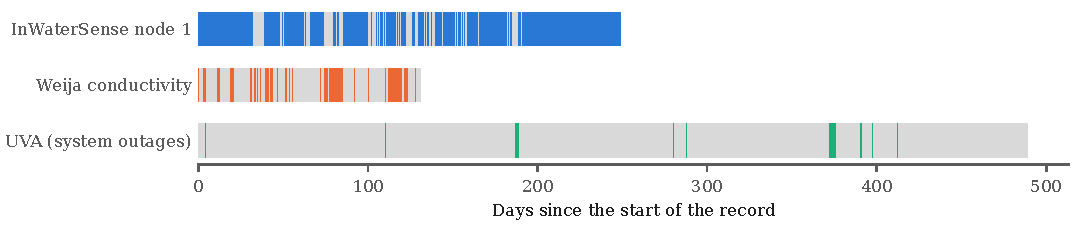
\includegraphics[width=\textwidth]{fig_records}
\caption{Delivery timelines of the three records with long gaps: coloured spans are slots in which nothing was delivered (UVA: system outages only; its short radio losses are not shown). Each record is drawn on its own time axis, from its first slot.}
\label{fig:records}
\end{figure*}

InWaterSense node~1 had \inwsOutages{} delivery gaps. Many were short: \inwsOneSlotEvents{} lasted a single slot, but together they held only \inwsOneSlotLost{} of the missing readings. At the other end, \inwsDayEvents{} gaps of a day or more (\inwsDayEventShare{} of all gaps) held \inwsDayLost{} of the missing readings (bootstrap 95\% CI \inwsDayLostLo--\inwsDayLostHi), and gaps of 6~h or more held \inwsSixLost{} (\inwsSixLostLo--\inwsSixLostHi). The longest lasted \inwsMaxOutageDays~days. Fig.~\ref{fig:outage-share} shows the whole curve.

The Weija deployment, on a different continent, shows the same structure. Its conductivity stream had \weijaCondOutages{} gaps and lost \weijaCondLoss{} of its readings; \weijaCondDayLost{} of the missing readings fell in gaps of a day or more, and the share was between \weijaDayLostMin{} and \weijaDayLostMax{} across all \weijaStreams{} streams, the longest gap lasting \weijaMaxOutageDays~days. With only \weijaCondDayN{} day-long gaps in the conductivity stream, its confidence interval is wide (\weijaCondDayLostLo--\weijaCondDayLostHi), so Weija is treated as qualitative support for the InWaterSense result rather than as a second estimate of it. As Sec.~\ref{sec:data-cause} showed, Weija's long gaps are silences of the whole node, and most of InWaterSense's long gaps were shared with the second node behind the same gateway.

\begin{figure}[t]
\centering
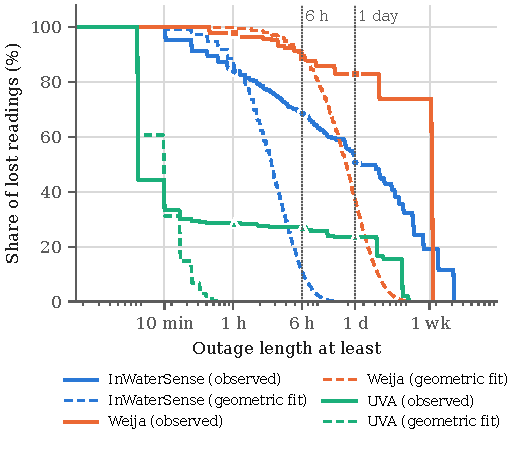
\includegraphics[width=\columnwidth]{fig_outage_share}
\caption{Share of missing readings that fall in gaps at least as long as the value on the horizontal axis, $S(L)$ in (\ref{eq:share}) (solid), and the same share predicted by the geometric model (\ref{eq:geo}) fitted to each record's gap lengths (dashed). Markers at 1~h, 6~h and 1~day. InWaterSense node~1 (611-s slots), Weija conductivity (\weijaCondStepMin-min slots) and UVA (all sensors, 5-min slots; radio and system losses together).}
\label{fig:outage-share}
\end{figure}

\subsection{The geometric gap-length model fails, and no tested model fits}
\label{sec:out-models}
Table~\ref{tab:aic} compares the four gap-length models (\ref{eq:geo})--(\ref{eq:pl}). The geometric model (\ref{eq:geo}), whose single loss state underlies both independent losses and the Gilbert--Elliott channel, ranks last on every record, by \aicGeomGapInws{} AIC points on InWaterSense, \aicGeomGapWeija{} on Weija and \aicGeomGapUva{} on UVA. Its failure is in exactly the quantity that matters, the long-gap share (\ref{eq:share}): fitted to InWaterSense, it puts \geomSixInws{} of the missing readings in gaps of 6~h or more, against \inwsSixLost{} observed, and \geomDayInws{} in gaps of a day or more, against \inwsDayLost{} (Fig.~\ref{fig:outage-share}). On Weija it puts \geomDayWeija{} in day-long gaps, against \weijaCondDayLost{}.
AIC only ranks the models, so each was also tested absolutely, by the bootstrap Kolmogorov--Smirnov test of Sec.~\ref{sec:data-outages}. The geometric model is rejected on every record ($p\le$\,\gofPmin, the smallest value the 200 bootstrap samples can give). With \gofInwsN{} gaps on InWaterSense and \gofUvaN{} runs on UVA, every tested model is rejected, but by very different margins: the geometric model's largest distance between fitted and observed distribution functions is \gofGeomDInws{} on InWaterSense and \gofGeomDUva{} on UVA, against \gofBestDInws{} and \gofBestDUva{} for the best of the other models. On Weija's few gaps, the lognormal and power-law models are not rejected ($p=$\,\gofWeijaLnP{} and \gofWeijaPlP). The ranking is not driven by one extreme gap: without the longest gap of each record, every record keeps its best model. A geometric gap-length model is thus strongly unsupported relative to the alternatives tested, and no tested model describes the larger records exactly.

No single alternative wins everywhere. The discrete lognormal is best by AIC on InWaterSense, the discrete power law on Weija (with the lognormal \aicWeijaLnGap{} AIC points behind), and the two-geometric mixture on UVA. The mixture's form, many short losses and a few long gaps, is the common thread, and the records differ visibly in how many long gaps they have (Fig.~\ref{fig:outage-share}). Gaps are also not independent of each other. On InWaterSense a long gap tends to be followed by another long gap (Spearman $\rho=$\,\inwsRhoNextOut) and by a short up-run ($\rho=$\,\inwsRhoNextUp; both \inwsRhoP), so gaps cluster into bad periods that a renewal model, drawing each gap independently, cannot reproduce. On Weija, with \weijaCondOutages{} gaps, neither correlation is distinguishable from zero ($\rho=$\,\weijaRhoNextOut, $p=$\,\weijaPNextOut; $\rho=$\,\weijaRhoNextUp, $p=$\,\weijaPNextUp). For these reasons all simulations in this paper replay the real records rather than a fitted model.

\begin{table}[t]
\centering
\caption{AIC of gap-length models (lower is better; best per record in bold). UVA: all missing-frame runs of all sensors, 5-min slots.}
\label{tab:aic}
\small
\begin{tabular}{@{}lrrr@{}}
\toprule
Model & InWaterSense & Weija & UVA \\
\midrule
\tabin{tables/tab_outage_models.tex}
\bottomrule
\end{tabular}
\end{table}

\subsection{LoRaWAN networks: short radio losses and rare system outages}
\label{sec:out-lorawan}
The two LoRaWAN records separate the causes of loss. On LoED, well-heard devices lost \loedRadioLoss{} of their frames to the radio. Losses were mildly bursty: the probability of losing a frame after a lost frame was \loedCondLoss, about \loedCondRatio{} times the marginal rate. But the bursts were short: of \loedBursts{} radio-loss bursts, \loedBurstOne{} were a single frame and \loedBurstFive{} at most five frames. Losses also did not coincide across devices beyond what their density implies: a lost frame coincided with a loss of another device at a shared gateway within the same minute in \loedCoLoss{} of cases, against \loedCoLossBase{} (\loedCoLossLo--\loedCoLossHi) under a random time-shift baseline.

UVA adds what LoED, recorded in campaign windows, cannot show: 16 months of continuous operation. The system as a whole was available \uvaAvail{} of the time, with \uvaSysOutages{} system outages (median \uvaSysMedianH~h, longest \uvaSysMaxH~h). Of the \uvaMissing{} missing frames, \uvaRadioShare{} were radio losses and \uvaSysShare{} system losses. The radio regime looks like LoED's: \uvaRunsOne{} of the \uvaRuns{} runs of missing frames were a single frame. The system regime looks like the water-quality deployments': \uvaSysDayShare{} of the system down-time fell in outages of a day or more. With few system outages, UVA's long outages hold a smaller share of its missing frames than at InWaterSense (\uvaSixLost{} in runs of 6~h or more, \uvaDayLost{} in runs of a day or more; Fig.~\ref{fig:outage-share}). The classification is not an artefact of the 10-minute bin: with bins of 5 to 30~min the number of system outages ranges from \uvaBinOutMax{} to \uvaBinOutMin{} (short ones merge), the share of system down-time in outages of a day or more from \uvaBinDayMin{} to \uvaBinDayMax{}, and the system share of missing frames from \uvaBinSysMin{} to \uvaBinSysMax{}.

Two further observations matter for design. First, \emph{gateway diversity masks gateway outages}: one of UVA's gateways was down for \uvaGwCDays{} days in a row, yet none of the missing frames was a gateway loss, because every sensor was also heard by a second gateway. Second, rain had no detectable effect on link loss: over \uvaRainPairs{} sensor--gateway pairs, loss was \uvaRainDry{} in dry hours and \uvaRainWet{} in rainy hours (Wilcoxon signed-rank test~\cite{wilcoxon1945individual}, $p=$\,\uvaRainP).

In answer to RQ1: across the four records studied, losses separate into short radio losses, which are nearly independent, and rarer long delivery gaps or system outages of a gateway, its backhaul, the server or the node. In the two water-quality deployments, gaps of 6~h or more hold most of the missing data (\inwsSixLost{} on InWaterSense, \weijaCondSixLost{} on Weija conductivity). A geometric gap-length model misses the second regime almost entirely.

\section{Retransmit or Backfill?}
\label{sec:handling}

The InWaterSense and Weija records were replayed as the link state for NB-IoT (search times \nbSearchTimes~s), LoRaWAN SF7, and LoRaWAN SF12, with and without independent radio losses: \nConfigs{} configurations in all. Table~\ref{tab:strategies} shows InWaterSense under the full-slot model; ranges are over all configurations, and further results are given in Supplementary Section~\ref{sec:s-handling}.

\begin{table*}[t]
\centering
\caption{Loss-handling strategies on the InWaterSense record (full-slot model, no added radio loss): transmission energy per day, $E_\mathrm{tx}$ in (\ref{eq:energy}), per radio (NB-IoT: $T_\mathrm{search}=10$~s), and the share of readings delivered and delivered within 1~h (LoRaWAN SF7; NB-IoT for the NB-IoT-only strategy). ARQ: LoRaWAN 1.0.2 behaviour. Back-off (\ref{eq:backoff}) capped at 6~h. --: not applicable.}
\label{tab:strategies}
\small
\begin{tabular}{@{}lrrrrr@{}}
\toprule
 & \multicolumn{3}{c}{Energy (J/day)} & \multicolumn{2}{c}{Readings} \\
\cmidrule(lr){2-4}\cmidrule(l){5-6}
Strategy & NB-IoT & SF7 & SF12 & Delivered & Within 1 h \\
\midrule
\tabin{tables/tab_strategies.tex}
\bottomrule
\end{tabular}
\end{table*}

\subsection{ARQ pays for losses it can hardly recover}
\label{sec:hand-arq}
Under the full-slot model, ARQ delivered exactly what unconfirmed reporting delivered, at \arqEightMin--\arqEightMax{} its energy on LoRaWAN with eight transmissions. This is the pessimistic end of a bracket. If the link may return during a gap's last slot, retries recovered \arqGainUniformMin--\arqGainUniformMax{} percentage points of InWaterSense's readings on LoRaWAN; if, in addition, gaps of up to an hour are radio-loss bursts, they recovered \arqGainBurstMin--\arqGainBurstMax{} points. Against the \arqLostPp{} points that unconfirmed reporting lost, ARQ thus recovered under a fifth in every model, at \arqRatioMin--\arqRatioMax{} the energy of unconfirmed reporting; on Weija, it recovered at most \arqGainWeijaMax{} points. NB-IoT ARQ recovered nothing because the modem reports that there is no network. LoRaWAN 1.0.4 (eight transmissions at a fixed rate) changed the price only slightly: \arqVOneZeroFour{} instead of \arqVOneZeroTwo{} at SF7. Retransmission suits the radio regime, not the long gaps that hold most of the missing data.

\subsection{Buffering buys completeness at a modest energy cost}
\label{sec:hand-buffer}
On NB-IoT, searching for a cell in every slot of a gap cost \backoffMin--\backoffMax{} the energy of backing off; thus, the fair NB-IoT baseline backs off. Against the fair baseline, confirmed reporting with a buffer and back-off delivered every generated reading at an energy change of \bufNbMin\% to \bufNbMax\% on NB-IoT and \bufLoMin\% to \bufLoMax\% on LoRaWAN. It was cheaper at SF7, where a confirmed success costs less than an unconfirmed report and the node stops transmitting into gaps, and more expensive at SF12. This completeness rests on three assumptions, each of which was tested:
\begin{enumerate}
\item The reading must exist: With up to half of the long-gap slots reassigned to a node that was off, buffering still delivered every generated reading, but only \offExpectedInws{} of the expected readings on InWaterSense.
\item The buffer must hold the backlog: The longest backlog was \maxBufferKB~KB; 2~KB of RAM lost \ramLossTwo{} of the readings and 64~KB none, and writing every reading to flash~\cite{winbond2018w25q128jv} cost at most \flashJDayMax~J/day.
\item The drain must leave room for live traffic: Limited to what the duty cycle leaves after one live frame per slot, the drain still delivered everything, but at SF12, a backlog persisted for \drainTwelveMaxD~days in InWaterSense's worst period; therefore, live readings should go ahead of the backlog~\cite{ingelrest2010sensorscope}.
\end{enumerate}

\subsection{Batching is cheaper and costs little timeliness}
\label{sec:hand-batch}
Hourly batching with buffer and back-off delivered every reading, while the fair per-reading baseline used \batchSaveMin--\batchSaveMax{} as much energy. Its share of readings within 1~h differed from that of unconfirmed reporting by only \batchWithinMin{} to \batchWithinMax{} points: under long gaps, the gaps, not the batch interval, decide how many readings arrive within the hour. The back-off cap trades energy against how long the server waits once the network is back. Probing every slot cost \kEverySlotSeven{} the energy of $K=6$~h at SF7, while raising $K$ to 24~h saved only \kSixToDaySave{} more and tripled the 90th-percentile wait (\kPninetySix{} to \kPninetyDay~h); $K=6$~h sits at this knee. The price of batching is the timeliness of alarms and of the real-time picture of fast parameters, which Section~\ref{sec:design} addresses.

\subsection{Many nodes and model uncertainty}
\label{sec:hand-network}
A system outage ends for every node behind the gateway simultaneously. A discrete-event model of one EU868 gateway and up to 500 nodes (collisions with capture, eight demodulators, a half-duplex gateway, and gateway duty cycles; Supplementary Table~\ref{tab:s-netsim}) showed two effects. Without randomisation, the deterministic back-off kept the nodes synchronised: from \netZeroJitterN{} nodes at SF7, almost none recovered within 72~h. With probes delayed randomly by up to an hour, every SF7 node recovered, the last within \netSevenAllMax~h, at up to \netSevenEnergyMax{} the energy of a node alone. At SF12, the gateway's acknowledgements ran out: its first-window sub-band reached its 1\% limit, up to \netTwelveNoAck{} of the received frames went unacknowledged, and after a one-day outage, only \netTwelveCleared{} of 100 nodes recovered within 72~h. The per-node results hold for cells with tens of nodes.

With every measured energy component multiplied by an independent factor between 1/2 and 2 (\mcDraws{} draws), ARQ cost more than unconfirmed reporting on LoRaWAN in \mcArqDearer{} of the draws. Hourly batching was cheaper than the fair baseline in at least \mcBatchCheapOther{} of them at SF7 and on NB-IoT, but only in \mcBatchCheapTwelveMin--\mcBatchCheapTwelveMax{} at SF12. The buffering energy relative to the fair baseline ranged from \mcBufLo{} to \mcBufHi{}, and its sign is set by the ratio of confirmed to unconfirmed energy, which can only be settled by measuring the target hardware.

In response to RQ2, ARQ recovers only the short radio losses under any timing model, and on LoRaWAN, it multiplies energy. Buffering with back-off recovers every generated reading, given tens of kilobytes of storage, at an energy close to that of recovering nothing in the model, and hourly batching is the energy-efficient way to do it at SF7 and on NB-IoT. Many nodes recovering simultaneously need randomised probes, and large SF12 cells are limited by the gateway's acknowledgements.

\section{Can Reconstruction Replace Delivery?}
\label{sec:reconstruct}

If a server could estimate the missing readings well enough, it would not need them delivered. This is tested on \chainCount{} river chains: sets of USGS gauging sites along the same river (Delaware, Illinois, Tualatin, Clackamas, McKenzie, Monongahela, Youghiogheny, Schuylkill and Klamath; \chainSites{} sites in all), each pair of sites on a chain serving as target and neighbour in both orders (\chainPairsMin--\chainPairsMax{} ordered pairs per parameter).

\subsection{Method}
All series are placed on a common 1-h grid. For every ordered pair, parameter and gap length (\chainGaps~h), gaps are simulated at the target (a median of \chainOutages{} per pair, parameter and length), drawn from the last 80\% of the year. A gap covers the slots after the last observed slot $t_0$ and before the next observed slot $t_1$. Let $y$ be the neighbour's series, lagged by $\ell$ hours, and $b$ a scaling slope; $\ell\in[0,48]$~h is chosen to maximise the correlation between 6-h changes of target and lagged neighbour in the first 20\% of the year, and $b$ is the least-squares slope of those changes (pairs whose best correlation is negative are dropped). \emph{Real-time} estimators use only data up to $t_0$, and the neighbour during the gap:
\begin{align}
\hat{x}_\mathrm{pers}(t)&=x(t_0), \label{eq:pers}\\
\hat{x}_\mathrm{diel}(t)&=x(t_0)+x(t-24\,\mathrm{h})-x(t_0-24\,\mathrm{h}), \label{eq:diel}\\
\hat{x}_\mathrm{nb}(t)&=x(t_0)+b\,[y(t)-y(t_0)], \label{eq:nb}\\
\hat{x}_\mathrm{dn}(t)&=\hat{x}_\mathrm{diel}(t)+b\,[y(t)-y(t_0)] \nonumber\\
&\quad-b\,[y(t-24\,\mathrm{h})-y(t_0-24\,\mathrm{h})]. \label{eq:dn}
\end{align}
Persistence (\ref{eq:pers}) holds the last value; own diel (\ref{eq:diel}) is the server's estimator (\ref{eq:picture}); neighbour change (\ref{eq:nb}) adds the neighbour's scaled change since the gap began; and diel + neighbour (\ref{eq:dn}) adds only the part of that change which the neighbour's own diel pattern does not explain. \emph{Bridging} estimators also know $x(t_1)$, as they would once backfilled data arrive:
\begin{align}
\hat{x}_\mathrm{int}(t)&=x(t_0)+\frac{t-t_0}{t_1-t_0}\,[x(t_1)-x(t_0)], \label{eq:int}\\
\hat{x}_\mathrm{in}(t)&=\hat{x}_\mathrm{int}(t)+b\,[y(t)-\bar{y}(t)], \label{eq:in}
\end{align}
where $\bar{y}$ is the straight line from $y(t_0)$ to $y(t_1)$, so that (\ref{eq:in}) adds the neighbour's departure from its own line to the interpolation (\ref{eq:int}). The error of an estimator on a gap is its maximum absolute error over the gap, $\max_{t_0<t<t_1}|\hat{x}(t)-x(t)|$; the median over gaps is reported, together with the share of gaps whose maximum error is within the L2 tolerance. Ordered pairs are not independent: a site appears in several pairs, and the pairs sit in \chainCount{} chains. Confidence intervals therefore resample whole chains, and pairs within each drawn chain (5{,}000 draws).

\begin{table*}[t]
\centering
\caption{Reconstruction on \chainCount{} river chains: median over ordered site pairs of the median maximum absolute error over a gap (T in $^\circ$C, DO in \%sat, pH in pH units, EC in $\mu$S/cm), and the share of pairs in which the neighbour improves on the target's own data. Real time: best neighbour method, (\ref{eq:nb}) or (\ref{eq:dn}), vs the better of persistence (\ref{eq:pers}) and own diel (\ref{eq:diel}). Bridging: interpolation + neighbour (\ref{eq:in}) vs interpolation (\ref{eq:int}).}
\label{tab:chains}
\small
\begin{tabular}{@{}lrrrrrrrr@{}}
\toprule
 & & \multicolumn{4}{c}{Real time} & \multicolumn{3}{c}{Bridging} \\
\cmidrule(lr){3-6}\cmidrule(l){7-9}
Param. & Gap (h) & Persistence & Own diel & Best neighbour & Neighbour wins & Interpolation & Interp.\ + neighbour & Neighbour wins \\
\midrule
\tabin{tables/tab_chains.tex}
\bottomrule
\end{tabular}
\end{table*}

\subsection{Results}
Table~\ref{tab:chains} gives the results for 1-h and day-long gaps. The text reports 24-h gaps; relative gains are medians over pairs, and exclude the \chainGainExcluded{} pH pairs whose target (site \chainExclSite) has a median error of exactly zero, for which a relative gain is undefined.

\emph{In real time, a site's own diel pattern is the estimator to beat.} It beats persistence in \chainDielBeatsPersistDo{} of pairs for DO and \chainDielBeatsPersistT{} for T. A neighbour improves on the better of the two own-data estimators in only \chainRtWinDo{} of pairs for DO (median gain \chainRtGainDo\%), \chainRtWinPh{} for pH (\chainRtGainPh\%) and \chainRtWinEc{} for EC (\chainRtGainEc\%). Temperature is the exception: a neighbour helps in \chainRtWinT{} of pairs (median gain \chainRtGainT\%), consistent with a shared, non-periodic weather driver.

\emph{When bridging a gap after the data return, the neighbour helps more.} The neighbour's shape improves interpolation in \chainBfWinT{} of pairs for T (median gain \chainBfGainT\%) and \chainBfWinDo{} for DO (\chainBfGainDo\%), but not for pH (\chainBfWinPh{} of pairs, \chainBfGainPh\%) or EC (\chainBfWinEc{}, \chainBfGainEc\%).

\emph{None of the six estimators keeps day-long gaps reliably within tolerance.} For 1-h gaps, the better own-data real-time estimator keeps a median of \chainTolOneH{} of gaps within the L2 tolerance. For 24-h gaps, even the best of all six, including the bridging ones that already know the value after the gap, keeps a median of only \recDayAll{} of gaps within tolerance (chain-resampled 95\% CI \recDayAllLo--\recDayAllHi; upper quartile of pairs \chainTolDayQ), from \recDayT{} for T to \recDayPh{} for pH.

\emph{A naive baseline overstates the value of neighbours.} Judged against persistence alone, a neighbour method wins in \chainNaiveWinDo{} of pairs for DO and \chainNaiveWinPh{} for pH, and the best neighbour method cuts the median DO error from \chainPersistDo{} to \chainBestNbDo~\%sat. Against the target's own diel pattern, which reaches \chainDielDo~\%sat, most of that gain disappears: the neighbour wins in \chainRtWinDo{} of DO pairs and \chainRtWinPh{} of pH pairs. Much of what a naive test credits to spatial correlation is the shared day--night cycle, which the target's own history already contains.

\emph{The fitted neighbour relation does not follow the flow.} The neighbours lie \pairKmMin{} to \pairKmMax~km from their targets (median \pairKmMed~km). If the neighbour carried water to the target, the selected lag would be positive for upstream neighbours and zero for downstream ones; instead, for DO a downstream neighbour gets a positive lag in \lagPosDown{} of pairs and an upstream one in \lagPosUp. The lag that maximises the correlation of 6-h changes tracks shared timing, of daylight and weather, rather than travel time. Evaluations of spatio-temporal reconstruction on river data therefore need a per-site diel baseline, and spatial structure taken from the river network rather than from correlation alone~\cite{peterson2010mixed}, a point also made for graph imputation in general~\cite{jing2024casper}.

\subsection{Contemporary deep imputers}
\label{sec:rec-deep}
The estimators above are deliberately simple. To test whether the conclusion is a limit of reconstruction or of these estimators, two contemporary deep imputers were added: SAITS, a self-attention model~\cite{du2023saits}, and StemGNN, a graph neural network that learns the relations between series~\cite{cao2020stemgnn} (implementations of PyPOTS; GRIN and SPIN need a graph library that the available machine could not hold). Each model sees all four parameters of every site of a chain in 192-h windows, normalised per window and series from the observed values, and is trained only on the first half of 2023 with masks that include whole-site blocks of 1--72~h, the evaluation scenario; the checkpoint with the best block error on a held-back part of the first half is kept. A first configuration, normalised with half-year means and spreads, under-fitted by an order of magnitude even on 1-h gaps and was discarded before any comparison. The models are tested on gaps drawn from the second half of the year, in which a whole site is missing for 1, 6, 24 or 72~h, and the paper's estimators are scored on the same \deepGaps{} gap--parameter cases. When bridging, they also see the data after the gap; in real time, nothing of the target after its start (the neighbours up to the end of the gap, which favours the deep models).

The deep imputers do not change the conclusion. On 1-h gaps they keep \deepBridgeOneSaits{} (SAITS) and \deepBridgeOneStem{} (StemGNN) of the cases within tolerance when bridging, against \deepBridgeOneInterp{} for interpolation, and \deepRtOneSaits{} and \deepRtOneStem{} in real time, against \deepRtOneDiel{} for the own-diel estimator. On day-long gaps they keep \deepBridgeDaySaits{} and \deepBridgeDayStem{} when bridging (interpolation: \deepBridgeDayInterp) and \deepRtDaySaits{} and \deepRtDayStem{} in real time (own diel: \deepRtDayDiel). Where they help is the error of DO and pH when bridging a day-long gap: SAITS's median maximum error is \deepDayDoSaits~\%sat for DO and \deepDayPhSaits{} for pH, against \deepDayDoInterp~\%sat and \deepDayPhInterp{} for interpolation, while it is worse for temperature and conductance. No estimator, simple or deep, keeps more than \deepDayBestAny{} of the day-long gaps of any parameter within tolerance.

In answer to RQ3, the reconstruction estimators evaluated, simple or deep, cannot replace delivery. For DO and pH the best real-time estimate is the site's own diel pattern, and neighbours add little; for temperature, and for bridging gaps after the data return, neighbours help, and a deep imputer reduces the DO and pH error. For gaps of a day, which hold most of the missing data in the water-quality records (Sec.~\ref{sec:outages}), none of the estimators keeps the error within tolerance in most gaps. Reconstruction's role is the interim estimate between deliveries, and only delivery restores the data. This is the role it plays in the design of Sec.~\ref{sec:design}.

\section{A Reporting Design and its Evaluation}
\label{sec:design}

Secs.~\ref{sec:outages}--\ref{sec:reconstruct} point to a design: buffer and back off through gaps (only delivery restores long gaps), batch routine data (cheap, and little less timely when gaps are long), and show the site's own diel estimate between deliveries. Batching leaves two gaps, alarms and the real-time picture of fast parameters, and the design closes them with two triggers that send a batch early.

\subsection{The design}
\label{sec:des-design}
\emph{Event-driven batching} runs at the node (Algorithm~\ref{alg:design}, without the bounded-error trigger). Every reading is buffered. Once an hour the node uploads its buffer in confirmed bulk frames. When the node's event detector raises an alarm, it uploads the buffer at once, alarming reading included; if the node is in an outage, an alarm triggers an immediate probe outside the back-off schedule (without resetting it). A failed upload puts the node into outage mode, with the probe back-off (\ref{eq:backoff}).

Fig.~\ref{fig:mechanism} shows these behaviours in a short illustrative scenario run through the simulator. Before the outage, the alarm makes the event-driven node upload at once, where plain batching would wait for the end of the hour; the alarm during the outage cannot get through; and after the outage, when the backlog arrives depends on where each strategy is in its back-off (\ref{eq:backoff}).

\begin{figure*}[t]
\centering
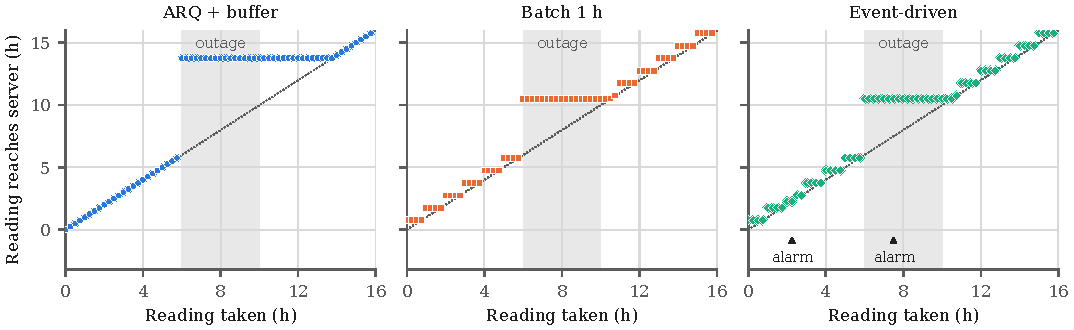
\includegraphics[width=\textwidth]{fig_mechanism}
\caption{When each reading reaches the server, in an illustrative scenario run through the simulator: LoRaWAN SF7, 15-min sampling, the link down from 6 to 10~h, and node alarms at 2.25~h (link up) and 7.5~h (link down). Points on the dotted diagonal arrive at once; horizontal runs are readings delivered together. Event-driven batching follows hourly batching except that the alarm at 2.25~h sends its batch early.}
\label{fig:mechanism}
\end{figure*}

\emph{Bounded event-driven batching} adds a \emph{bounded-error trigger}. Because every upload is confirmed, the node knows which of its readings have reached the server and when; it can therefore compute, at every slot $t$, the value $\hat{x}_j(t)$ that the server is showing for each parameter $j$, by evaluating (\ref{eq:picture}) on the readings it knows to have arrived. It uploads its buffer at once (Algorithm~\ref{alg:design}) if
\begin{equation}
\max_{j}\ \frac{|x_j(t)-\hat{x}_j(t)|}{\delta_j}>1,
\label{eq:trigger}
\end{equation}
that is, if any parameter's true reading differs from what the server shows by more than its tolerance $\delta_j$. This is the dual-prediction mechanism of error-bounded report suppression~\cite{dias2016survey,santini2006adaptive}, used here to bound the error between batches rather than to suppress reports. Three details matter. First, the trigger is not consulted during an outage: the server's estimate may drift far from the truth during a long gap, and a node that probed every time would waste energy on a dead link; only alarms probe. Second, the node's copy of the server must model \emph{when} readings arrive, not only \emph{whether}: on LoRaWAN the duty cycle spaces the frames of a long upload, so a reading enters $A(t)$ in (\ref{eq:picture}) only after its frame's arrival time, and the newest valid reading goes in the first frame of every upload, so that the value the server most needs arrives first. Third, the node's knowledge of the server comes from acknowledgements, so it is only as good as their boundary. On NB-IoT the confirmation is the application server's reply~\cite{michelinakis2021dissecting}, and the node knows what the server holds. On LoRaWAN a confirmed uplink is acknowledged by the network server; the forwarding to the application server, which UVA's ``system'' losses show can fail, is not covered. A variant of the trigger closes this gap at a cost (Sec.~\ref{sec:des-ack}): it keeps the bound for both possible server states, with and without the readings the network server acknowledged, until an application acknowledgement returns in the downlink of a later uplink.

\begin{algorithm}[t]
\caption{Bounded event-driven batching: node, one slot}
\label{alg:design}
\small
\begin{algorithmic}[1]
\State append the slot's reading $x_t$ to the buffer
\If{in outage mode}
  \If{alarm at $t$ \textbf{or} back-off timer expired} \State probe; on success leave outage mode and upload the buffer \EndIf
  \State \Return
\EndIf
\State $\hat{x}(t) \gets$ server's estimate (\ref{eq:picture}), from readings whose arrival time is $\le t$
\If{alarm at $t$ \textbf{or} trigger (\ref{eq:trigger}) \textbf{or} hour boundary}
  \State upload the buffer (newest valid reading first), confirmed bulk frames
  \State on failure enter outage mode, back-off (\ref{eq:backoff})
\EndIf
\end{algorithmic}
\end{algorithm}

\subsection{Evaluation protocol}
\label{sec:des-protocol}
\emph{Two phases.} The design was developed on 2023 data and then tested on held-out 2024 data. In the development phase, hypotheses H1--H4 and their decision rules were written down before the runs for event-driven batching; after H4 failed, H5--H7 were written for the bounded-error trigger before it was implemented, and H8--H10, on packing order and on the tolerance level, before they were run. Every deviation was recorded when made, with its reason: UVA replayed as system outages plus radio losses (D1); one site excluded because its eligibility had been computed over its record span rather than the year (D2); seeds derived from site identifiers (D3); two implementation defects of the packing order, which made H8 fail as written (D4); and a floating-point tie at the tolerance (D5, found during the revision): pH and T are recorded in 0.1 steps, and an error of exactly one tolerance was counted in or out by rounding noise, in the scores and in the trigger. All development results below are from a rerun with D4 and D5 fixed. For the confirmatory phase, the final design, the analysis code, its decision rules and the eligibility rule were frozen, and the code identified by cryptographic hashes, before any 2024 data were downloaded; the 2024 verdicts below are the output of that frozen code. The plans are kept with the code and hashed; they were not registered with a third party.

\emph{Sites.} Every USGS site of the \designCandidates{} candidates with all four parameters in complete cycles for at least half of the year: \designSites{} sites in 2023 and \confSites{} in 2024 (\sitesBothYears{} in both years). Sampling steps are 5 to 60~min. The first 20\% of each record trains the detector; all metrics are computed on the remaining 80\%.

\emph{Links.} The no-outage link, and three real records mapped onto each site's time grid in physical time, wrapped circularly with a random start offset per site (seeded by the site identifier, with a different seed in 2024): InWaterSense and Weija conductivity, in which every missing slot is a down link (the full-slot model, pessimistic for the per-reading strategies), and UVA, replayed as its system outages plus independent radio losses at the rate of a representative sensor (\uvaSensorFourRadio{} per attempt). \emph{Radios:} NB-IoT ($T_\mathrm{search}=10$~s), LoRaWAN SF7 and SF12.

\emph{Strategies.} Unconfirmed, ARQ + buffer, hourly batching (``batch 1~h''), event-driven batching, and bounded event-driven batching (newest-first packing, L2 tolerance unless stated), as defined above and in Sec.~\ref{sec:data-energy}.

\emph{Injected events.} Events are added to the real test-period series, so background dynamics, noise and gaps are real and only the event is synthetic. For parameter $j$, let $a_j(t)$ be the reading minus its centred 24-h running median, and $r_j(t)$ that anomaly minus its median for the same calendar month and hour of day. The event scale is the robust standard deviation of $r_j$ in the event's month,
\begin{equation}
\sigma_j=\max\left(1.4826\,\operatorname{MAD}\!\left[r_j\right],\ \rho_j\right),
\label{eq:scale}
\end{equation}
floored at the recording resolution $\rho_j$, estimated from the data as the most common positive difference between sorted distinct values. An event of amplitude $\kappa\sigma_j$, with $\sigma_j$ from (\ref{eq:scale}), $\kappa\in\{5,8\}$ and a random sign, lasts 180~min: a \emph{step} adds $\kappa\sigma_j$ for its whole duration, and a \emph{ramp} rises linearly from 0 to $\kappa\sigma_j$; injected values are rounded to $\rho_j$. Events touch one parameter each, in turn, lie in the test period, at least a day after the start of a data segment and wholly inside it, and at least three days apart (at most 60 per site and setting; \designEventsConf{} in 2024). The events are of a realistic size. Their median amplitudes are mild in physical units (5$\sigma$/8$\sigma$: T \ampFiveT/\ampEightT~$^\circ$C, DO \ampFiveDO/\ampEightDO~\%sat, EC \ampFiveEC/\ampEightEC~$\mu$S/cm, pH \ampFivePh/\ampEightPh), and real 3-hour changes of at least 5$\sigma$ occur at \realFiveT{} of the sites for T, \realFiveDO{} for DO, \realFiveEC{} for EC and \realFivePh{} for pH (8$\sigma$: \realEightT, \realEightDO, \realEightEC, \realEightPh). They are physically plausible: \plausibleConf{} of the 2024 events stay within T $-0.5$--40~$^\circ$C, positive EC, pH 4--11 and DO 0--250~\%sat (\plausibleDev{} in 2023).

\emph{Detector.} All strategies use the same causal detector: on the node for the event-driven designs, and on the server, on the readings it has received, for the others. It compares each reading with the reading $m=120$~min earlier, corrected by a learned hour-of-day profile $p(\cdot)$ of the departure from the running 24-h median, and runs a two-sided CUSUM~\cite{page1954continuous} on the clipped, standardised residual:
\begin{align}
z_t&=\operatorname{clip}\!\left(\frac{x_t-x_{t-m}-p(h_t)+p(h_{t-m})}{s},\,-c,\,c\right),\label{eq:z}\\
S^{+}_t&=\max\left(0,\,S^{+}_{t-1}+z_t-k\right),\nonumber\\
S^{-}_t&=\max\left(0,\,S^{-}_{t-1}-z_t-k\right),\label{eq:cusum}
\end{align}
where $h_t$ is the hour of day and $s$ a robust residual scale floored at $\rho_j$. An alarm is raised when either sum in (\ref{eq:cusum}), driven by the residual (\ref{eq:z}), exceeds $H$, with $k=3$, $H=8$ and $c=6$; the detector then stays in an event state until $|z_t|<2$ for 60~min, and resets its sums. The profile and the scale are initialised on the training period and updated by exponential smoothing (memory about 7~days) only outside the event state. These parameters were fixed before any evaluation and were not tuned on its data. An event counts as detected if an alarm on its parameter occurs during it. In 2024 the detector caught a median (over sites) of \detectStepFive{} of 5$\sigma$ steps, \detectStepEight{} of 8$\sigma$ steps, \detectRampFive{} of 5$\sigma$ ramps and \detectRampEight{} of 8$\sigma$ ramps (\detectAll{} of all events), with a median of \faMedian{} false alarms per parameter per 30 days (mean \faMean).

\emph{Metrics.} \emph{Alarm latency}: the time from an event's onset to the arrival of its alarm at the server, for detected events, split by whether the link was up at onset. Because an operator cares about the whole chain, the share of \emph{all} injected events that the server knows of within 1, 6 and 24~h is also reported. \emph{Energy}: transmission J/day, $E_\mathrm{tx}$ in (\ref{eq:energy}), including uploads caused by alarms and false alarms; for the event-driven designs, averaged over the four event settings. \emph{Picture}: the share of scored slots at which the server's real-time picture (\ref{eq:picture}) is within tolerance, on the series without injected events. Each is summarised as the median over sites per link and radio (12 link--radio combinations; 48 with the four parameters), with 95\% confidence intervals from resampling sites (10{,}000 draws).

Table~\ref{tab:hyp} lists the hypotheses and their verdicts in both phases.

\begin{table*}[t]
\centering
\caption{Hypotheses, decision rules and verdicts. Each rule applies to the median site of every link--radio combination (12), or of every link--radio--parameter combination (48), and passes only if it holds in all. Phase of writing: P, before the development runs; A, after H4 failed, before the runs concerned. Development: 2023 rerun with D4 and D5 fixed; held-out: 2024, judged by the frozen code. ``Event'' = event-driven batching; ``Bounded'' = bounded event-driven batching.}
\label{tab:hyp}
\small
\begin{tabular}{@{}llp{5.0cm}p{4.6cm}ll@{}}
\toprule
 & & Claim & Rule & 2023 (development) & 2024 (held-out) \\
\midrule
H1 & P & Link up: Event raises alarms as fast as per-reading reporting & Event $-$ ARQ+buffer alarm latency $\le$ 1 slot & Pass, \chOneDev & Pass, \chOneConf \\
H2 & P & Event costs about as much as batching, much less than per-reading ARQ & Event / batch $\le 1.10$ and ARQ+buffer / Event $\ge 1.3$ & Pass, \chTwoDev & Pass, \chTwoConf \\
H3 & P & Onset in an outage: buffering delivers late, unconfirmed loses & descriptive & As expected & As expected \\
H4 & P & Event's picture is as good as per-reading reporting's & Event $\ge$ ARQ+buffer $-$ 5 pp & Fail, \chFourDev & Fail, \chFourConf \\
H5 & A & Bounded's picture is as good as per-reading reporting's & Bounded $\ge$ ARQ+buffer $-$ 1 pp & Pass, \chFiveDev & Pass, \chFiveConf \\
H6 & A & Bounded costs no more than per-reading ARQ & Bounded $\le$ ARQ+buffer energy & Pass, \chSixDev & Pass, \chSixConf \\
H7 & A & The trigger does not delay alarms & Bounded $-$ Event alarm latency $\le$ 1 slot & Pass, \chSevenDev & Pass, \chSevenConf \\
H8 & A & Newest-first packing makes the picture exact with the link up & 100\% within tolerance, no outage, every site & Fail as written; pass after D4 & Pass \\
H9 & A & H5 holds at tolerances L1 and L3 & as H5 & Pass, \chNineLOneDev, \chNineLThreeDev & Pass, \chNineLOneConf, \chNineLThreeConf \\
H10 & A & H6 holds at tolerances L1 and L3 & as H6 & Pass, \chTenLOneDev, \chTenLThreeDev & Pass, \chTenLOneConf, \chTenLThreeConf \\
\bottomrule
\end{tabular}
\end{table*}

\subsection{Alarms with the link up (H1, H7)}
\label{sec:des-alarms}
With the link up at an event's onset, event-driven batching raises alarms at the server as fast as per-reading ARQ in both years (H1; Table~\ref{tab:design}). The median latency of about an hour is the detector's own: the CUSUM needs about an hour of evidence, and delivery adds nothing. Plain hourly batching is slower in every combination, by a median of \batchLagMinConf--\batchLagMaxConf~h in 2024. On the InWaterSense link the event-driven design is never slower than ARQ + buffer, and faster at SF12 in 2024 (on every radio in 2023), because an alarm probes at once while ARQ + buffer waits for its back-off schedule when a gap starts during the event. The bounded-error trigger does not delay alarms (H7). Counting all injected events, detected or not, the server knows of \knownOneEventNoneConf{} within an hour with event-driven batching on the no-outage link at SF7, the same as with per-reading reporting, against \knownOneBatchNoneConf{} with hourly batching; within a day it knows of \knownDayEventNoneConf{} with any of them. On the InWaterSense link the shares within an hour are \knownOneBoundedInwsConf{} (bounded), \knownOneArqInwsConf{} (ARQ + buffer), \knownOneUnconfInwsConf{} (unconfirmed) and \knownOneBatchInwsConf{} (batch), and within a day \knownDayBoundedInwsConf, \knownDayArqInwsConf, \knownDayUnconfInwsConf{} and \knownDayBatchInwsConf. The ceiling is the detector's \detectAll{} detection, not the reporting scheme.

\begin{table}[t]
\centering
\caption{Held-out year (2024): alarm latency with the link up (median over sites of each site's median, hours) and transmission energy (median over sites, J/day); LoRaWAN SF7. Energies of the event-driven designs are averaged over the four event settings. ARQ: ARQ + buffer.}
\label{tab:design}
\scriptsize
\setlength{\tabcolsep}{2.2pt}
\begin{tabular}{@{}lrrrrrrrr@{}}
\toprule
 & \multicolumn{4}{c}{Alarm latency (h)} & \multicolumn{4}{c}{Energy (J/day)} \\
\cmidrule(lr){2-5}\cmidrule(l){6-9}
Link & ARQ & Batch & Event & Bounded & ARQ & Batch & Event & Bounded \\
\midrule
\tabin{tables/tab_design.tex}
\bottomrule
\end{tabular}
\end{table}

\subsection{Energy (H2, H6)}
\label{sec:des-energy}
Alarm uploads are rare (a median of \alarmsPerDay{} alarms per node per day in 2024; mean \alarmsPerDayMean), and most ride on readings that would have been sent within the hour anyway. Event-driven batching therefore costs \eventOverBatchMinConf--\eventOverBatchMaxConf{} as much as plain batching, and ARQ + buffer costs \arqOverEventMinConf--\arqOverEventMaxConf{} as much as event-driven batching (H2). The bounded-error trigger costs more, \boundedOverBatchMinConf--\boundedOverBatchMaxConf{} the energy of plain batching, because each trigger sends an extra upload between batches. Per-reading ARQ still uses \arqOverBoundedMinConf--\arqOverBoundedMaxConf{} as much energy as the bounded design (H6; every site-resampled 95\% interval lies above \arqOverBoundedCiLowConf), against \arqOverBoundedMinDev--\arqOverBoundedMaxDev{} in the development year. At an hourly cadence an hourly batch holds a single reading, so batching cannot save energy there.

\subsection{The real-time picture (H4, H5)}
\label{sec:des-picture}
Table~\ref{tab:picture} and Fig.~\ref{fig:tradeoff} show the server's picture. Plain event-driven batching fails H4 in both years: for DO, an estimate up to an hour old leaves the L2 tolerance between batches, and the picture is \hFourFailMinConf{} to \hFourFailMaxConf{} percentage points less often within tolerance than with per-reading reporting (2023: \hFourFailMinDev{} to \hFourFailMaxDev). The failures occur with no outage at all, so they are a property of hourly batching, not of the gaps. The event detector does not help: these excursions are ordinary diel motion, not events. (In the first development run, H4 also failed for pH, \hFourPassVOne{} combinations passing; the pH failures were the rounding tie D5, not batching.)

The bounded-error trigger removes the failure. The bounded design's picture is within \hFiveDiffMinConf{} to \hFiveDiffMaxConf{} percentage points of per-reading reporting's for every parameter, link and radio (H5; 2023: \hFiveDiffMinDev{} to \hFiveDiffMaxDev). With the link up and no radio loss it is within tolerance at every scored slot, by construction (H8 below).

Under the two water-quality gap records, unconfirmed reporting shows a \emph{better} picture than ARQ + buffer for every parameter and radio (e.g., DO on InWaterSense at SF7: \picInwsDoUnconf{} vs \picInwsDoArq). When the link returns, an unconfirmed node delivers its next reading at once, while a buffering node waits for its next back-off probe. The back-off saves energy and costs timeliness right after gaps; unconfirmed reporting, of course, never delivers the readings lost in them.

\begin{table}[t]
\centering
\caption{Held-out year (2024): share of scored slots within the L2 tolerance (median over sites; LoRaWAN SF7; series without injected events). ARQ: ARQ + buffer.}
\label{tab:picture}
\scriptsize
\setlength{\tabcolsep}{3pt}
\begin{tabular}{@{}llrrrrr@{}}
\toprule
Link & Param. & Unconf. & ARQ & Batch & Event & Bounded \\
\midrule
\tabin{tables/tab_picture.tex}
\bottomrule
\end{tabular}
\end{table}

\begin{figure*}[t]
\centering
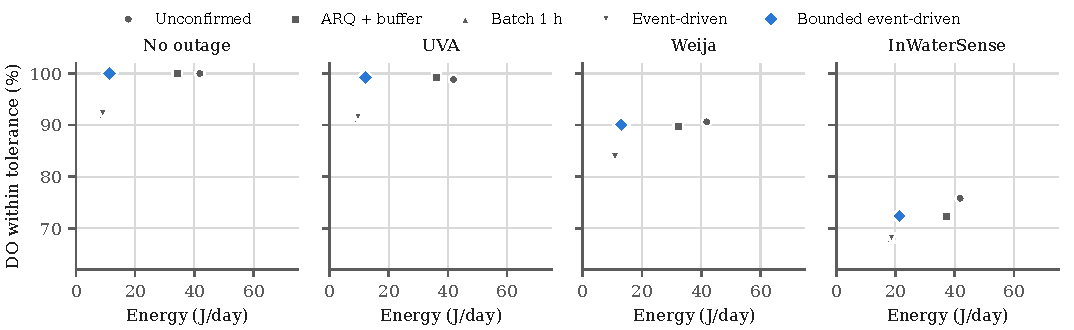
\includegraphics[width=\textwidth]{fig_tradeoff}
\caption{Held-out year (2024): energy against the real-time picture of DO (share of slots within the L2 tolerance), LoRaWAN SF7, median over sites, one panel per link, all panels on the same vertical scale. Batch~1~h and event-driven batching nearly coincide. The bounded design reaches the picture of per-reading reporting at a fraction of its energy.}
\label{fig:tradeoff}
\end{figure*}

\subsection{Events that start during a gap (H3)}
\label{sec:des-outage}
Table~\ref{tab:onset} and Fig.~\ref{fig:onset} show the detected events whose onset fell in a gap. As expected (H3), every strategy has to wait for the link. Unconfirmed reporting learns of almost none of these events (at most \onsetUnconfKnownMax{} on any link and radio): the alarming readings fall inside the gap and are lost. The buffering strategies learn of at least \onsetBufKnownMin, but only after the gap; the gap, not the reporting scheme, sets this latency. Within it, the immediate alarm probe makes the event-driven designs faster than ARQ + buffer on the water-quality records.

\begin{table}[t]
\centering
\caption{Held-out year (2024): detected events whose onset fell in a gap (LoRaWAN SF7, pooled over sites): number of events, share the server ever learns of, and median latency of those it learns of (hours).}
\label{tab:onset}
\scriptsize
\setlength{\tabcolsep}{2.4pt}
\begin{tabular}{@{}lrrrrrrrr@{}}
\toprule
 & & \multicolumn{3}{c}{Known ever} & \multicolumn{4}{c}{Median latency (h)} \\
\cmidrule(lr){3-5}\cmidrule(l){6-9}
Link & $n$ & Unconf. & ARQ & Event & ARQ & Batch & Event & Bounded \\
\midrule
\tabin{tables/tab_onset.tex}
\bottomrule
\end{tabular}
\end{table}

\begin{figure*}[t]
\centering
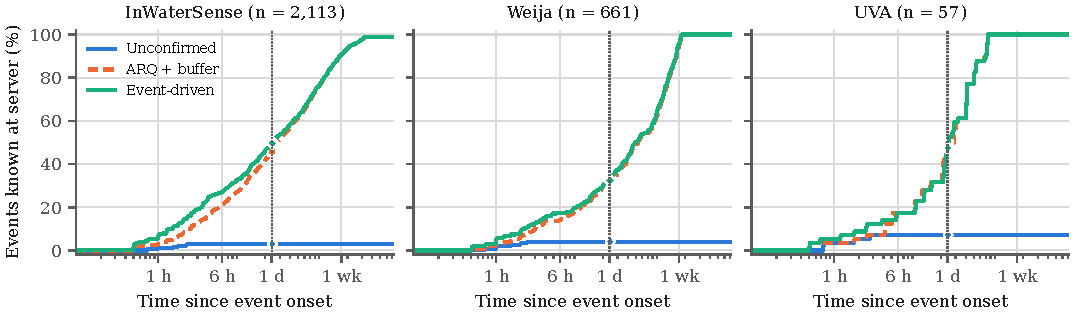
\includegraphics[width=\textwidth]{fig_outage_onset}
\caption{Held-out year (2024): detected events whose onset fell in a gap, share known at the server by the time on the horizontal axis (LoRaWAN SF7, pooled over sites; markers at 1~day). Unconfirmed reporting learns of almost none; the buffering strategies learn of nearly all, after the gap.}
\label{fig:onset}
\end{figure*}

\subsection{Packing order and tolerance level (H8--H10)}
\label{sec:des-sens}
On SF12 a frame holds only \rpfSfTwelve{} readings, so an hourly batch at 15-min sampling needs two frames, and the duty cycle delays the second. With first-in-first-out packing the newest reading rode in the second frame, and in the first development run the server's picture on the no-outage link fell to \fifoMinSfTwelve{} at worst instead of 100\%. H8 predicted that packing the newest reading first would make it exact everywhere. As written, H8 failed: the picture fell short at one site (\hEightPreSite, 5-min sampling, SF12), with a minimum of \hEightPreMin{}. The cause was two implementation defects, each a departure from the stated design: the reading promoted to the first frame could be a placeholder for a sensor gap rather than the newest valid reading, and the node's copy of the server counted readings as known as soon as their upload began, although at 5-min sampling an SF12 upload spans several slots. Both were fixed (D4); the lesson is general: a node that mirrors its server must model when data arrive, not only whether. With the fix, newest-first packing is within tolerance at every scored slot of the no-outage link, on every site, parameter and radio, in both years, at \nfRatioMin--\nfRatioMax{} times the energy of first-in-first-out packing (2024).

The tolerance level sets the price of the bound (Table~\ref{tab:sensitivity}). The picture stays within 1 percentage point of per-reading reporting at every level (H9), and per-reading ARQ uses \levOneArqOverMinConf--\levOneArqOverMaxConf{} the bounded design's energy at L1, \levTwoArqOverMinConf--\levTwoArqOverMaxConf{} at L2 and \levThreeArqOverMinConf--\levThreeArqOverMaxConf{} at L3 (H10).

\begin{table}[t]
\centering
\caption{Held-out year (2024): energy (median J/day over sites, LoRaWAN SF7, series without injected events) at three tolerance levels, the median over sites of each site's ARQ / Bounded energy ratio, and the lowest within-tolerance share over the four parameters (median site). ARQ: ARQ + buffer.}
\label{tab:sensitivity}
\scriptsize
\setlength{\tabcolsep}{2.5pt}
\begin{tabular}{@{}llrrrrr@{}}
\toprule
 & & \multicolumn{2}{c}{Energy (J/day)} & & \multicolumn{2}{c}{Within tolerance} \\
\cmidrule(lr){3-4}\cmidrule(l){6-7}
Level & Link & ARQ & Bounded & ARQ/Bounded & Bounded & ARQ \\
\midrule
\tabin{tables/tab_sensitivity.tex}
\bottomrule
\end{tabular}
\end{table}

\subsection{Where the server's state comes from}
\label{sec:des-ack}
On LoRaWAN, the evaluation above takes a confirmed uplink's acknowledgement, which comes from the network server, as proof that the application server shows the reading. If the node may not assume this, it keeps the bound for both possible server states until an application acknowledgement returns in the downlink of a later uplink (Sec.~\ref{sec:des-design}). On the development sites, this costs \ackCostMin{} to \ackCostMax{} more energy than trusting the network server, because the node uploads again whenever the older state could be out of tolerance; the picture of the median site stays within \ackPicWorst{} percentage points of per-reading reporting, and per-reading ARQ still uses \ackArqOverMin--\ackArqOverMax{} as much energy. On NB-IoT the question does not arise: its confirmation is the application's reply.

The answer to RQ4 is yes, with the link up, and on data not used to design the scheme. Bounded event-driven batching delivers every reading the node generates, raises alarms as fast as per-reading reporting, keeps the server's picture within a chosen tolerance as often as per-reading reporting does, and costs \boundedOverBatchMinConf--\boundedOverBatchMaxConf{} the energy of plain hourly batching, while per-reading ARQ uses \arqOverBoundedMinConf--\arqOverBoundedMaxConf{} as much energy on the held-out year. What no scheme can fix is the gap itself: events and data during a gap reach the server only when the link returns.

\section{Discussion}
\label{sec:discussion}

\subsection{Practical guidance}
\label{sec:disc-guidance}
The results suggest six rules for battery-powered water-quality telemetry on LPWANs.

(1)~\emph{Know which regime loses your data.} Short radio losses and long delivery gaps call for different remedies, and in the two water-quality deployments studied the long gaps held most of the missing data. A delivery log with frame counters, a note of when the gateway and server were down, and the node's own status are enough to tell the regimes and their causes apart (Secs.~\ref{sec:data-cause} and \ref{sec:outages}). Simulations and estimators that assume geometric gap lengths should be checked against such a log.

(2)~\emph{Do not fight long gaps with retransmissions.} ARQ is useful against radio losses only; under any of the timing models it recovers under a fifth of the readings missing in the long-gap record. Confirm, buffer and back off instead; on NB-IoT, back off even if nothing is buffered, because searching for a cell in every slot of a gap cost up to \backoffMax{} the energy of backing off in the swept range (Sec.~\ref{sec:handling}).

(3)~\emph{Give the buffer room and the backlog manners.} Tens of kilobytes held the longest backlog in these records, and writing it to flash costs almost nothing. At high spreading factors the duty cycle, not the buffer, limits recovery: interleave live readings ahead of the backlog. Where many nodes share a gateway, randomise the recovery probes, and at SF12 acknowledge backlogs in chunks rather than frame by frame (Sec.~\ref{sec:hand-network}).

(4)~\emph{Batch routine data, and make the batch leave early when it matters.} Hourly batching delivers every reading for a fraction of per-reading energy at SF7 and on NB-IoT; at SF12 its advantage depends on the energy of a confirmed frame and should be measured. Two triggers close its two gaps: an event alarm, for timeliness, and a bounded-error trigger that mirrors the server's estimate, for the real-time picture. The tolerance is then the operator's energy knob, and a tolerance at the USGS ``excellent'' accuracy of the sensors costs well under the energy of per-reading ARQ (Sec.~\ref{sec:design}). The node must model when its data arrive, and, on LoRaWAN, whether the application has them.

(5)~\emph{Use the site's own diel pattern as the interim estimate, and judge reconstruction against it.} Between deliveries, a site's own day--night pattern is the best simple estimator for DO and pH; neighbours help temperature, and help most when bridging a gap after the data return. A reconstruction method evaluated only against the last value will overstate what spatial information adds (Sec.~\ref{sec:reconstruct}).
Contemporary deep imputers, trained per river, reduce the error of DO and pH when bridging a day-long gap, but keep fewer short gaps within tolerance than the simple estimators and no more day-long ones (Sec.~
ef{sec:rec-deep}).

(6)~\emph{Engineer the gaps themselves.} No reporting scheme shortens a gap; events that start during one reach the server only when it ends. Gateway diversity masked a month-long gateway outage at UVA without losing a frame (Sec.~\ref{sec:out-lorawan}), and deployment reports show that watchdog resets bound how long silent gateway failures last~\cite{brzozowski2018lessons,ingelrest2010sensorscope}. How long system outages last is partly an operations variable.

\subsection{Validity and limitations}
\label{sec:disc-limits}
\emph{Delivery records.} The loss evidence comes from two water-quality deployments and two LoRaWAN networks; it supports statements about these records, not a law for all deployments. The Weija record has few long gaps and serves as qualitative support only, and its unflagged interpolation hides some short gaps. The cause of a gap could be checked only partly (Sec.~\ref{sec:data-cause}); buffering's recovery is therefore an upper bound, tested with up to half of the long-gap slots reassigned to a node that was off. UVA's ``system'' outages include the operators' own logging pipeline, which from a user's point of view is still data that did not arrive.

\emph{Energy without hardware.} No hardware was built for this study. The energy model rests on published measurements of specific modules and network settings, with an ideal battery, and an independent measurement on a different board and stack differs from it severalfold in absolute terms (Sec.~\ref{sec:data-energy}). The results are therefore ratios between strategies on the same radio, tested against a factor-of-two uncertainty on every measured component (Sec.~\ref{sec:hand-robust}); lifetimes are illustrative. The energy an NB-IoT modem spends searching when there is no network has no published measurement that could be found, so it was swept. A measurement campaign on a LoRaWAN and an NB-IoT node, including a deliberate gateway disconnection, is the most important next step.

\emph{What the per-node model leaves out.} Clock faults, reordering and storage failure~\cite{murphy2021arctic,brzozowski2018lessons} are not simulated. Many nodes recovering at once are studied with a separate, simplified model of one gateway (Sec.~\ref{sec:hand-network}); multi-gateway reception, adaptive data rate and real channel conditions would change its numbers, but not the two mechanisms it shows, synchronised probes and acknowledgement capacity.

\emph{Events and detection.} The events are synthetic steps and ramps injected into real series, of realistic size and physically plausible, and the detector, whose parameters were fixed in advance, catches slow ramps poorly (\detectRampFive{} of 5$\sigma$ ramps). The latency comparisons concern how fast the server learns of a detected event; the all-event shares show how much of an operator's view is set by detection rather than by reporting.

\emph{Rivers and tolerances.} The river data cover two years in one country, and some lower-Delaware sites are tidal, where conductivity follows the tide rather than the day. The held-out year shares most sites with the development year (\sitesBothYears{} of \confSites), so it tests the design on new data, not on new rivers. The tolerances are at or inside the USGS accuracy ratings, not regulatory limits; the sensitivity analysis shows how the results change with them. The server's estimator is deliberately simple, and a learned estimator could shorten the bounded design's extra uploads, but not the gap a long outage leaves.

\emph{Pre-specification.} The development hypotheses and decision rules were written down before their runs and kept with the code; the confirmatory plan and code were frozen and hashed before the held-out data were downloaded. Neither was registered with a third party. Every verdict is reported, including the failures and the defect found during the revision (D5), with its effect.

\subsection{Conclusion}
In the four records studied, data are lost in two regimes: short radio losses, and rarer long delivery gaps that, in the two water-quality deployments, hold most of the missing data. Remedies designed for short, independent losses fit the first regime and not the second. Retransmission spends energy on gaps it cannot bridge, and the reconstruction estimators evaluated, from a site's own history to deep imputers, keep most day-long gaps outside the tolerance. Buffering with back-off delivers every reading the node generates at an energy close to that of not recovering at all, and hourly batching makes it cheaper still. A reporting design that batches hourly, sends alarms at once, and leaves early whenever the server's estimate would leave tolerance matched per-reading reporting on alarm latency and on the real-time picture on a held-out year of river data, while per-reading ARQ used \arqOverBoundedMinConf--\arqOverBoundedMaxConf{} as much energy. The remaining gap is the outage itself, which only network engineering, such as gateway diversity and watchdogs, can shorten. Future work includes hardware measurements of the design, longer and tropical outage records, the energy of NB-IoT cell search without a network, and recovery of many nodes across several gateways.


\section*{Data and Code Availability}
The USGS~\cite{usgs2023nwis}, InWaterSense~\cite{ahmedi2021inwatersense}, LoED~\cite{bhatia2020loeddata} and UVA~\cite{nikseresht2025uvadata} data are public. The Weija records were provided by the deployment's operators~\cite{adumanu2020smart}; their raw values are not redistributed, but the delivery trace derived from them (the time of every record of every stream, and whether it counts as a genuine delivery) is. The code, configurations, seeds, environment lock files, data-acquisition scripts, input checksums, the frozen confirmatory plan with the hashes of the frozen code, and the derived traces are archived at [archive DOI].  % to be inserted at submission Every number in this paper is generated from the result files by a script that records its source.

\section*{Acknowledgment}
This work received no external funding.

\bibliographystyle{IEEEtran}
\bibliography{refs}

\end{document}
